% ============================================================
% Momentum, Breadth, and Correlation in Tactical Asset Allocation: A Rule-by-Rule Attribution
% Authors: Garcia Martin I., Mases Campos M., Prior Sanz F.
% Institution: IQS School of Engineering, Universitat Ramon Llull
% Target: International Review of Economics & Finance (IREF, Elsevier)
% ------------------------------------------------------------
% Elsevier elsarticle submission draft.
%   [review]  -> double-spaced, single-column, line numbers (for referees).
% For the final typeset version switch [review] to [final,5p] (or [final,1p]).
% The previous article-class working draft is preserved in git history.
% ============================================================
\documentclass[review,12pt]{elsarticle}

% elsarticle loads natbib internally; do NOT load natbib/authblk again.
\usepackage{amsmath, amssymb}
\usepackage{amsthm}
\usepackage{booktabs}
\usepackage{graphicx}
\usepackage{float}
\usepackage{longtable}
\usepackage{multirow}
\usepackage{array}
\usepackage[T1]{fontenc}
\usepackage[utf8]{inputenc}
\usepackage{xcolor}
\usepackage{enumitem}
\usepackage[hidelinks]{hyperref}

% author-year citations to match the existing \citep/\citet calls
\biboptions{round,authoryear}

\newcolumntype{R}[1]{>{\raggedleft\arraybackslash}p{#1}}

% Theorem environments
\newtheorem{proposition}{Proposition}
\newtheorem{lemma}{Empirical Regularity}

\journal{International Review of Economics \& Finance}

% ============================================================
\begin{document}

\begin{frontmatter}

\title{Momentum, Breadth, and Correlation in Tactical Asset
Allocation: A Rule-by-Rule Attribution}

\author[iqs]{Ignasi Garcia Martin}
\author[iqs]{Marc Mases Campos}
\author[iqs]{Francesc Prior Sanz\corref{cor1}}
\ead{francesc.prior@iqs.url.edu}
\cortext[cor1]{Corresponding author.}

\affiliation[iqs]{organization={IQS School of Engineering, Universitat Ramon Llull},
            addressline={Via Augusta 390},
            postcode={08017},
            city={Barcelona},
            country={Spain}}

% ---- Abstract -----------------------------------------------
\begin{abstract}
We design and evaluate a fully automated, rule-based tactical asset allocation
(TAA) strategy that rotates monthly across a diversified universe of 15
exchange-traded funds (ETFs), without leverage, derivatives, or discretionary
intervention.
The strategy combines four components: a multi-period (13612U) momentum score,
a top-$7$ breadth pre-filter, an absolute-momentum threshold with a
breadth-based defensive switch, and a minimum-correlation triplet selection rule.
The primary focus is a transparent, rule-by-rule attribution of the strategy's
out-of-sample edge rather than the strategy itself.

ETF histories are extended back to 2003 using documented proxies (underlying
indices or calibrated instruments with $R^2 \geq 0.92$) and a strict nested
temporal split is adopted: three parameters are derived on a 2004--2015 training
window and confirmed on a 2016--2020 validation window, while the absolute
threshold is fixed ex ante at the risk-free rate; the frozen strategy is then
evaluated once on a locked 2021--2025 test block.
On the test block the strategy attains a CAGR of 11.42\%, a Sharpe ratio of
0.873, and a maximum drawdown of $-7.06\%$; over the full 2004--2025 period it
attains 11.00\%, 0.892, and $-11.86\%$.

A matched-permutation test finds that the momentum rule beats a random matched
baseline on the Sharpe ratio ($p = 0.0025$) and the minimum-correlation rule
contributes through variance reduction (variance ratio $1.28$, $p = 0.010$)
rather than return; a nested spanning-alpha ladder shows the edge arises from
stacking complementary rules.
The resulting spanning alpha against $1/N$ on the locked test is $+6.9\%$ per
annum ($p = 0.008$), survives joint controls for equity, duration, and a
time-series-momentum factor, and passes a Deflated Sharpe ratio correction at
$0.975$.
\end{abstract}

\begin{keyword}
Tactical asset allocation \sep momentum \sep minimum-correlation portfolios \sep
drawdown control \sep data snooping \sep spanning regressions \sep ETF rotation \sep
out-of-sample validation
\end{keyword}

\end{frontmatter}

% ============================================================
% ============================================================
\section{Introduction}
\label{sec:introduction}
% ============================================================

Rule-based tactical asset allocation (TAA) strategies are popular precisely
because they are transparent: an allocation is driven by a handful of explicit
rules (a momentum signal, a ranking cutoff, an absolute-trend filter, a
portfolio-construction criterion) rather than by an opaque optimiser.
Momentum, the workhorse signal of these rules, is one of the most robust
regularities in asset markets, both cross-sectionally and as a time-series effect
across asset classes \citep{jegadeesh1993, moskowitz2012, asness2013}.
Yet that same transparency raises a question the literature rarely answers head on.
Among the several rules a typical strategy stacks, which ones actually generate the
out-of-sample edge, which are inert, and is the whole thing anything more than a
repackaged time-series-momentum (trend) premium? Without an answer, a favourable
backtest is hard to tell apart from the product of a parameter search
\citep{yang2019, harvey2018}.

This paper takes one concrete cross-asset momentum strategy and treats it as a case
study for exactly that question. We derive each rule on a locked training window and
then decompose its out-of-sample performance rule by rule. The tools are a
matched-permutation (skill-versus-luck) test and a nested spanning-alpha ladder, and
we then put the residual edge through controls for known risk factors (including a
trend factor built from the same assets), transaction costs, a multiple-testing
adjustment, and a replication on 100\% real data. The strategy itself is designed
under a hard drawdown-control objective, which we keep as the evaluation criterion.
But the contribution is the attribution, not the strategy.

The strategy under study combines four components.
First, a multi-period (13612U) momentum score averages 1-, 3-, 6-, and 12-month
signals to reduce dependence on any single lookback horizon.
Second, a top-$7$ breadth pre-filter restricts the candidate set to the
higher-momentum half of the universe.
Third, an absolute-momentum threshold defines an eligible set and drives a
breadth-based defensive switch: when fewer than three assets clear the threshold,
the cross-section of momentum has broadly deteriorated and the portfolio rotates
to long- and intermediate-duration treasuries, or to cash if bond momentum is also
negative \citep{keller2017, antonacci2014}.
Fourth, a minimum-correlation triplet selection rule implements the central
diversification insight of modern portfolio theory \citep{markowitz1952} by
holding the three lowest-correlation assets among the eligible candidates.
Regime detection is thus driven by the \emph{breadth of momentum} (the count of
assets clearing the absolute threshold) rather than by a separate market-return
trigger.

We evaluate the strategy on a universe of 15 diversified ETFs covering global
equities, real estate, commodities, and fixed income; exchange-traded funds make
systematic multi-asset rotation operationally feasible by providing liquid,
low-cost exposure to broad asset classes.
Because the ETFs were launched between 2002 and 2008, a real-ETF backtest is too
short for a powered train/validation/test design; we therefore extend each series
back to 2003 using documented proxies (underlying indices or OLS-calibrated
correlated instruments), with the data-construction choices and their limitations
reported in Section~\ref{sec:methodology}.
The empirical design uses a strict nested temporal split: the momentum signal, the
breadth count, and the triplet size are derived on the 2004--2015 training window
(each lands on its ex-ante literature value) and confirmed on a 2016--2020
validation window, while the absolute threshold is fixed ex ante at the risk-free
rate rather than optimised; the frozen strategy is then evaluated once on a locked
2021--2025 test block. Supporting robustness analyses are reported over the broader
post-training sample (2016--2025) for statistical power.
The out-of-sample windows span the COVID-19 crash (validation) and the 2022
inflation and rate shock and 2023--2025 recovery (test).

The main result is that the strategy delivers competitive risk-adjusted returns
with materially lower drawdowns than passive benchmarks.
Over the full 2004--2025 period it achieves a CAGR of 11.00\%, a Sharpe ratio of
0.892, and a maximum drawdown of $-11.86\%$.
On the locked test block (2021--2025) it achieves a CAGR of 11.42\%, a Sharpe ratio
of 0.873 (the highest of the benchmark panel), and a maximum drawdown of $-7.06\%$,
roughly one-third that of $1/N$ ($-23.8\%$), 60/40 ($-21.1\%$), and the S\&P~500
($-24.8\%$).

The paper makes three contributions.
The central one is a transparent, two-pronged attribution
framework for rule-based TAA strategies, deployed here on a concrete four-rule
strategy as a case study. The framework combines a matched-permutation
(skill-versus-luck) test, which replaces each rule's informed decision with a random
draw from the same feasible set, with a nested incremental spanning-alpha ladder
that isolates each rule's marginal out-of-sample contribution. The resulting
decomposition is more informative, and more defensible against
data-snooping charges, than either a single in-sample optimisation or an aggregate
out-of-sample test. Applied to GAT, it finds that the momentum rule beats its
matched random baseline ($p = 0.0025$); the minimum-correlation rule contributes
through variance reduction (variance ratio $1.28$, $p = 0.010$) rather than
through return; and the remaining parameters, fixed ex ante in flat regions of the
objective, are statistically indistinguishable from random matched choices. The
incremental ladder tells the same story. No single rule is individually significant
in isolation; the edge emerges from stacking complementary rules, and the
combination is what generates the alpha.
The second contribution is a formal and empirical account of the minimum-correlation
construction. Proposition~\ref{prop:mincorr} shows analytically that, within a
momentum-screened eligible set with homogeneous expected returns, the
minimum-average-correlation triplet is the minimum-variance equal-weight portfolio.
The data then show that this is precisely its empirical role. It compresses
portfolio variance and tail risk at statistically equal expected
return and without inverting a covariance matrix, so the gain is risk control rather
than return. Reporting a null return contribution
alongside a significant risk contribution is, we argue, an honest finding with direct
implications for anyone designing multi-rule TAA systems: the rule earns its
place through drawdown compression, not alpha.
The third contribution is breadth of evidence for the spanning alpha.
The locked test block delivers $+6.9\%$ per annum against $1/N$ ($p = 0.008$) and
a residual of $+4$--$5\%$/yr against joint controls for equity, duration, and a
long-only time-series-momentum factor built from the same 15 assets. That long-only
factor is the hardest appropriate control for a long-only strategy, and GAT still
clears it ($+7.6\%$/yr against
TSMOM$_{\text{LO}}$, $p = 0.018$; $+4.3\%$ against the standard long-short
TSMOM, $p = 0.04$, both on the locked test). The rest of the robustness battery
points the same way. Realistic transaction costs (break-even
$\approx 62$ bps against $10\times$/yr turnover), temporal stability, universe
perturbation, a Deflated Sharpe ratio of $0.975$, and a replication on 100\% real
ETF data each fail to overturn the result. We also confront the strategy's main
practical weakness, its tax inefficiency relative to buy-and-hold: the tax drag is
real ($\approx 3$ percentage points of annual return), yet GAT retains the highest
after-tax Sharpe of the benchmark panel (Section~\ref{sec:res_tax}).
The strategy itself is transparent, reproducible, and implementable with monthly
ETF trades, but our central message is methodological: the attribution framework
reveals where a rule-based TAA edge comes from and, equally important, where it
does not.

The remainder of the paper is structured as follows.
Section~\ref{sec:literature} reviews the relevant literature.
Section~\ref{sec:methodology} describes the strategy design and data.
Section~\ref{sec:results} reports in-sample performance, the rule-by-rule
attribution, out-of-sample and full-period results, and the robustness battery.
Section~\ref{sec:discussion} discusses what the attribution implies about the
source of the edge.
Section~\ref{sec:conclusion} concludes.

% ============================================================
\section{Literature Review}
\label{sec:literature}
% ============================================================

The strategy builds on five interconnected bodies of evidence. We set them out in the order they inform the design.

The core signal is momentum. \citet{jegadeesh1993} document that past equity winners outperform past losers over intermediate horizons, and \citet{asness2013} extend the evidence across asset classes and geographies. \citet{moskowitz2012} establish the time-series counterpart: an asset's own past return predicts its future return across equities, bonds, currencies, and commodities. A survey by \citet{jegadeesh2023} confirms both effects remain robust three decades on. A practical difficulty in applying momentum is that no single lookback horizon dominates consistently across assets and periods: short windows capture reversals rather than continuation, while very long windows can capture mean-reversion. The 13612U signal in Rule~1 addresses this by averaging 1-, 3-, 6-, and 12-month excess returns, blending horizons known to carry cross-sectional and time-series momentum in approximately equal measure \citep{moskowitz2012, keller2017}. The pre-filter in Rule~2 restricts candidates to the top-$7$ assets by this score before the absolute threshold is applied: concentrating the eligible set on the highest-momentum names reduces exposure to assets near the boundary of positive momentum and has been shown to improve return and drawdown outcomes in multi-asset rotation \citep{faber2007, keller2017}. Several papers have translated the momentum insight into ETF-based rotation strategies: \citet{faber2007} shows that a moving-average rule materially reduces drawdowns in a diversified asset portfolio; \citet{blitz2008} apply value and momentum across asset classes; \citet{clare2016} combine trend following and risk-parity ideas in global allocation; and \citet{bellu2020} propose a momentum framework with explicit cash protection in downturns, the closest published precedent to our strategy. More recent work by \citet{wouassom2022} and \citet{vukovic2023} documents momentum in international equity markets. The present paper shares this lineage but differs in focus: rather than evaluating a strategy as a whole, it attributes out-of-sample performance rule by rule.

\citet{antonacci2014} formalises the combination of cross-sectional and absolute momentum as \emph{dual momentum}: assets are first ranked relative to peers, then screened against a positive-trend threshold. The absolute filter is the cash-protection mechanism, preventing the portfolio from holding assets in a downtrend regardless of relative rank. \citet{antonacci2012} and \citet{antonacci2015} provide supporting empirical evidence. Our Rule~3 retains only assets whose 13612U score exceeds the cash rate ($\theta = 2\%$), directly implementing this filter, and the breadth-based defensive switch extends the same logic to the portfolio level: when momentum collapses broadly, the portfolio exits risky assets entirely.

\citet{keller2017} extend the absolute-momentum concept to a \emph{breadth} signal: the fraction of assets with positive momentum serves as a regime indicator for the Vigilant and Hybrid Asset Allocation frameworks. Breadth-based switching is well motivated by \citet{daniel2016}, who show that momentum crashes cluster in panic states where most assets deteriorate simultaneously, and by \citet{barroso2015}, who document that momentum is most vulnerable precisely when volatility is elevated. Triggering the defensive switch through breadth collapse uses the same signals that drive offensive allocation, making regime detection endogenous and fully auditable.

When selecting a small portfolio from a large eligible set, the covariance structure matters. \citet{markowitz1952} establishes diversification as the mechanism for reducing portfolio risk; in practice, however, estimating the full covariance matrix for a large universe introduces substantial estimation error. \citet{demiguel2009} demonstrate that naive equal-weight ($1/N$) allocation is hard to beat net of this error, a result that motivates our equal-weight design. Once an absolute momentum filter has been applied, the eligible assets share similar expected returns (as we verify on the training data), so the only remaining lever for portfolio construction is their correlation structure: selecting the lowest-correlation triplet minimises portfolio variance while bypassing matrix inversion. This rule-based, estimation-light approach is the portfolio-theoretic foundation of Rule~4. Neither \citet{faber2007} nor \citet{keller2017} incorporate a correlation-based selection criterion within the eligible set; once assets pass the absolute filter, both frameworks weight them equally without regard to their pairwise correlations. The minimum-correlation triplet is the feature that most directly differentiates the present strategy from this prior work, and characterising its precise role through a skill-versus-luck attribution is the paper's central question.

The flexibility of rule-based backtests makes them vulnerable to data snooping. \citet{sullivan1999} and \citet{white2000} formalise this concern for technical trading rules; \citet{harvey2016} document pervasive multiple-testing bias in the cross-section of expected returns; and \citet{bailey2014} propose the Deflated Sharpe Ratio as a multiple-trial correction. \citet{yang2019} apply these cautions directly to tactical allocation rules. The existing literature typically delivers a snooping-corrected verdict on a strategy as a whole. It less often asks which rule inside the strategy carries the edge. We bring the two together, attributing performance rule by rule through a skill-versus-luck permutation test and a nested spanning-alpha ladder. The combination localises the edge and, at the same time, offers a constructive defence against the snooping critique.

% ============================================================
\section{Methodology}
\label{sec:methodology}
% ============================================================

This section develops the design of the TAA strategy as a sequential derivation
of rules from the stated objective, rather than as a fixed algorithm.
The objective is to maximise the Sharpe ratio subject to a soft
drawdown target of no worse than $-15\%$.
Each design choice is either derived on the training window
(February~2004 -- December~2015) or, for the absolute threshold, fixed ex ante from
the literature; the choices are then confirmed on a separate validation
window (2016--2020) and only then locked; the test window (2021--2025)
is evaluated exactly once, after all parameters are frozen
(Section~\ref{sec:data}).
We show in Section~\ref{sec:robustness} and in the empirical results
that the two parameters that drive performance (the momentum signal and the
minimum-correlation rule) cannot be reproduced by chance, whereas the remaining
parameters sit in flat regions of the training objective and coincide with values
fixed ex ante in the literature, so they could not have been overfit.

%-------------------------------------------------------------
\subsection{Problem Formulation and Constraints}
\label{sec:formulation}
%-------------------------------------------------------------

Let $V_t$ be the portfolio value at end of month $t$ and
$r_{f,t}$ the monthly 3-month U.S.\ Treasury Bill return.
The design problem is:

\begin{equation}
\max_{\boldsymbol{\Theta}}\;\text{Sharpe}_{T_{\text{train}}}(\boldsymbol{\Theta})
\quad \text{subject to} \quad
\text{MaxDD}_{T_{\text{train}}}(\boldsymbol{\Theta}) \gtrsim -15\%
\label{eq:problem}
\end{equation}

where $\boldsymbol{\Theta}$ is the set of design parameters and $T_{\text{train}}$
indexes the training sample.
The constraint formalises a capital-preservation requirement that temporary
losses remain limited; it takes precedence over return maximisation.
The Sharpe ratio is computed from monthly excess returns over the T-bill rate
(Section~\ref{sec:metrics}); all robustness analyses use the same convention.

The investment universe consists of 15 risky ETFs spanning six geographic equity
regions, real estate, commodities, and fixed income, plus one cash proxy
(Table~\ref{tab:universe}).

\begin{table}[H]
\centering
\caption{Investment universe}
\label{tab:universe}
\small
\begin{tabular}{llll}
\toprule
ETF & Name & Asset Class & Region \\
\midrule
SPY & SPDR S\&P 500 & Equity & US Large Cap \\
QQQ & Invesco QQQ & Equity & US Technology \\
VGK & Vanguard FTSE Europe & Equity & Europe \\
EWJ & iShares MSCI Japan & Equity & Japan \\
SCZ & iShares MSCI EAFE Small Cap & Equity & Intl Small Cap \\
EEM & iShares MSCI Emerging Markets & Equity & Emerging Markets \\
VNQ & Vanguard Real Estate & Real Estate & US REITs \\
REM & iShares Mortgage Real Estate & Real Estate & US Mortgage REITs \\
GLD & SPDR Gold Shares & Commodity & Gold \\
IEF & iShares 7--10 Year Treasury & Fixed Income & US Intermediate \\
TLT & iShares 20+ Year Treasury & Fixed Income & US Long Duration \\
TIP & iShares TIPS Bond & Fixed Income & US Inflation-Linked \\
DBC & Invesco DB Commodity Index & Commodity & Broad Commodities \\
BWX & SPDR Bloomberg Intl Treasury & Fixed Income & International \\
RWX & SPDR Dow Jones Intl Real Estate & Real Estate & Intl REITs \\
\midrule
BIL & SPDR Bloomberg 1--3 Month T-Bill & Cash Proxy & US Cash \\
\bottomrule
\end{tabular}
\end{table}

%-------------------------------------------------------------
\subsection{Data, Sample, and the Nested Derivation Protocol}
\label{sec:data}
%-------------------------------------------------------------

\paragraph{Universe construction.}
The 15 risky assets were selected before any backtest was performed, following the
standard multi-asset ETF panel used in the TAA literature
\citep{faber2007, antonacci2014, keller2017}: broad equity regions (US large-cap,
technology, Europe, Japan, international small-cap, emerging markets), real estate
(US REITs and mortgage REITs), commodities (gold and a broad commodity index), and
fixed income (intermediate and long US Treasuries, TIPS, international bonds, and
international real estate). This universe was fixed at the outset; no assets were
added or removed after inspecting backtest results. The leave-one-out robustness
analysis (Section~\ref{sec:res_robustness}) confirms that no single asset is
necessary for the result.

The 16 instruments were launched between 2002 and 2008, so a backtest on real ETF
data alone does not begin cleanly until around 2008 ($\approx 214$ months), too
short to support a three-way train/validation/test split with adequate power in
each segment.
To extend the history we reconstruct each series back to 2003 using documented
proxies: the underlying index where available, or an OLS-calibrated correlated
instrument, spliced to the ETF at its launch date following the procedure of
\citet{keller2017}.
For each asset we estimate $r_{\text{ETF}} = \alpha + \beta\, r_{\text{proxy}} +
\varepsilon$ over the overlapping sample, apply
$r_{\text{cal}} = \alpha + \beta\, r_{\text{proxy}} - \text{ER}/12$ to the pre-ETF
window (where $\text{ER}$ is the ETF's annual expense ratio, subtracted in monthly
terms so that the synthetic series reproduces the fund's net-of-fee return), and
rebuild the price series; bond ETFs are reconstructed from yields via a
constant-maturity total-return formula ($R^2 > 0.99$ against the realised ETF). The
proxy, its source, the calibration $R^2$, and the splice window for every asset are
listed in Appendix~\ref{app:data}.

Every risky asset is tracked by real ETF data, by its exact underlying index, or
by a high-$R^2$ calibrated proxy. Five series use real ETF data throughout the live
window (SPY, QQQ, EWJ, IEF, TLT); three use the exact benchmark the ETF replicates
(VNQ via the MSCI US REIT index, SCZ via MSCI EAFE Small Cap, RWX via the Dow Jones
Global ex-US Select RESI, all $R^2 \geq 0.92$); the remainder use near-exact or
high-$R^2$ proxies (gold futures for GLD, $R^2 = 0.99$; the S\&P GSCI for DBC,
$R^2 = 0.90$; a European country-ETF composite for VGK, $R^2 = 0.96$; and the T.\
Rowe Price International Bond fund for BWX, $R^2 = 0.94$). Two segments fall below
$R^2 = 0.90$: the 2003--2006 portion of the mortgage-REIT series (REM), proxied by a
three-name mortgage-REIT basket ($R^2 = 0.80$) until its sector index becomes
available ($R^2 = 0.94$ from 2006), and the 11-month pre-launch warm-up of TIP
(January--November~2003, $R^2 = 0.40$), which precedes the strategy's live window
and is never used in a momentum signal computation. REM rarely enters the final
triplet. Full proxy details, sources, and splice windows are in
Appendix~\ref{app:data}.

\paragraph{Nested train/validation/test protocol.}
The 12-month warm-up of the 13612U signal makes February~2004 the first live
month, leaving 263 monthly returns through December~2025. We split them
chronologically into three blocks and treat them in a strict nested protocol:
\begin{itemize}
    \item \textbf{Training} (2004:02--2015:12, 143 months, $\approx 54\%$):
          every parameter in $\boldsymbol{\Theta}$ is derived here by a
          grid search that maximises the in-sample Sharpe of
          Equation~\eqref{eq:problem}.
    \item \textbf{Validation} (2016:01--2020:12, 60 months, $\approx 23\%$):
          where a training-optimal value differs from the value suggested by the
          literature, the candidate is selected on this out-of-sample block;
          a training pick that does not survive validation is reverted to its
          literature value. No test data are observed at this stage.
    \item \textbf{Test} (2021:01--2025:12, 60 months, $\approx 23\%$):
          the frozen strategy is evaluated once; this is the paper's primary
          inferential claim (Table~\ref{tab:oos}). The test block spans the 2022
          inflation/rate shock and the 2023--2025 recovery.
\end{itemize}
Three of the four parameters are derived: for each we locate the training
optimum, then check the validation block for catastrophic failure before freezing.
For the signal, the breadth count, and the triplet size, the training optimum
coincides with the ex-ante literature value (13612U, $N=7$, $k=3$;
Sections~\ref{sec:signal}--\ref{sec:topn}, \ref{sec:triplet}).
Parameters are locked by the training optimum alone; the validation block
serves as a sanity check (did the training pick collapse out of sample?) rather
than as a selection criterion. None of the three training picks fails validation:
the dominant choice (13612U, $N=7$, $k=3$) is in each case unambiguous in the
143-month training window and consistent with the literature, so validation adds
no degree of freedom and the test block is fully held out. The 60-month validation
block taken in isolation occasionally elevates a different value (e.g.\ $k=2$) by
a margin well within its sampling noise; we note this explicitly as evidence that
the training pick is \emph{not} validated on a short window and then projected into
the test, but rather locked before the validation block is observed.
The threshold is treated differently and deliberately: it is fixed ex ante at
the long-run risk-free rate ($\theta=2\%$), following \citet{antonacci2014}, rather
than optimised. We are explicit that the in-sample objective does \emph{not} single
out $2\%$: on an unrestricted grid the training and pooled Sharpe are flat-to-noisy
in $\theta$ and peak at a higher value (train+validation Sharpe $0.938$ near
$\theta=4.5\%$ versus $0.897$ at $2\%$). We do not adopt that in-sample maximum: the
threshold has a clear economic anchor (an asset trending below cash carries no
expected premium), and selecting the higher in-sample value would be precisely the
data snooping the protocol is designed to avoid. As Section~\ref{sec:theta} shows,
the $2\%$ floor is what secures the strategy's drawdown control, and the result is
robust across the threshold band. The
supporting robustness analyses
(Section~\ref{sec:robustness}) are reported over the broader post-training sample
(2016--2025, 120 months) and the full sample (2004--2025) for statistical power,
and are clearly labelled as such.

\paragraph{Declared limitations of the data construction.}
Two features are stated openly because a rigorous reader will require them.
\emph{(i) Calibration look-ahead.} Because several ETFs (BIL, SCZ, REM, BWX) were
launched only in 2007, their sole overlap for OLS calibration falls inside the
training window; the synthetic pre-2007 returns therefore use coefficients fitted
partly on later data within the same training block. The effect is bounded: it
touches only the early training segment (2004--2007), the validation and test
blocks are 100\% real ETF data, and every proxied series now uses its exact
underlying index or a proxy with $R^2 \geq 0.92$ (the lone exception, REM's
2003--2006 basket, rarely enters the final triplet). As an external check
(Section~\ref{sec:res_robustness}), the same strategy run on a 100\% real-ETF
sample (2009--2025, no proxies) yields a consistent alpha ($+6.04\%$/yr,
$p = 0.0001$), indicating that the proxy calibration is not the source of the edge.
\emph{(ii) Momentum warm-up.} The dataset begins in January~2003 and the 13612U
signal needs twelve months, so all of 2003 is forced to cash; the live training
window is therefore 2004--2015.

%-------------------------------------------------------------
\subsection{Rule 1: Momentum Signal}
\label{sec:signal}
%-------------------------------------------------------------

\textit{Design question}: which momentum signal best captures cross-sectional
predictability over the training period?

The momentum score of each asset is the equal-weight average of its 1-, 3-, 6-,
and 12-month total returns (the ``13612U'' specification of \citealp{keller2017}):

\begin{equation}
M_{i,t}^{\text{13612U}} = \frac{1}{4}\left(R_{i,t}^{1} + R_{i,t}^{3} + R_{i,t}^{6} + R_{i,t}^{12}\right)
\label{eq:momentum}
\end{equation}

where $R_{i,t}^{k}$ is the $k$-month compound return of asset $i$ ending at $t$.
We compare 13612U against single-horizon (1m, 3m, 6m, 12m), blended (6--12,
3--6--12), and weighted (13612W) alternatives by training-window Sharpe.
On the extended training window 13612U is the in-sample Sharpe optimum
(0.865, ahead of the best single horizon at 0.814 and the weighted 13612W at
0.629), and it is the specification advocated ex ante by the literature
\citep{moskowitz2012, asness2013, keller2017}. Adopting a value that is
simultaneously the training optimum and the ex-ante literature choice removes it as
a source of overfitting.

%-------------------------------------------------------------
\subsection{Rule 2: Universe Filtering (Top-$N$)}
\label{sec:topn}
%-------------------------------------------------------------

\textit{Design question}: how many assets should enter the candidate set?

Assets are ranked in descending order of $M_{i,t}$; the top $N$ form the
candidate set. We evaluate $N \in \{1,\ldots,12\}$ on the training period.
On the extended 143-month training window the in-sample Sharpe is maximised at
exactly $N = 7$ (Sharpe 0.865), the value implied ex ante by the
$\approx 50\%$-of-universe heuristic of \citet{faber2007} and the
\citet{keller2017} HAA framework. The training optimum and the literature value
coincide, so $N = 7$ is set without a degree of freedom to overfit.

%-------------------------------------------------------------
\subsection{Rule 3: Absolute Threshold $\theta$ and Breadth-Based Defensive Switch}
\label{sec:theta}
%-------------------------------------------------------------

\textit{Design question}: should all top-ranked assets be held, and what happens
when the cross-section of momentum deteriorates?

Rank-based momentum selects the best assets relative to the universe but
does not prevent holding assets in a negative absolute trend.
Following \citet{antonacci2014}, we impose an absolute threshold: only assets with
$M_{i,t} \geq \theta$ pass from the Top-$N$ candidate set into the eligible set:

\begin{equation}
\mathcal{A}_t^+ = \left\{i \in \text{Top-}N_t \;\big|\; M_{i,t} \geq \theta \right\}
\label{eq:eligible}
\end{equation}

Unlike the other parameters, the threshold is fixed ex ante rather than
optimised: following \citet{antonacci2014} we set $\theta = 2\%$, approximately the
long-run risk-free rate, on the economic grounds that an asset trending below cash
carries no expected premium. We are deliberately transparent that the in-sample
objective does not pin down this value. Over an unrestricted grid
($\theta \in \{0\%, 0.5\%, \ldots, 5\%\}$) the training Sharpe is flat-to-noisy in
$\theta$ and in fact peaks at a higher threshold (training Sharpe $0.924$ at
$\theta=5\%$, pooled train+validation $0.938$ near $\theta=4.5\%$, versus $0.865$ and
$0.897$ at $\theta=2\%$); a search would therefore have selected a higher floor. We
do \emph{not} adopt the in-sample maximum, since doing so would tune the threshold to
the sample, precisely the data snooping the nested protocol is designed to avoid;
we keep the economically anchored value instead.
\emph{Procedural note.} The threshold was fixed at $\theta = 2\%$ before the test
block was examined. The decision sequence was: (i) derive $\theta$ on the training
grid and note the flat-to-noisy profile peaking at $\approx 4$--$5\%$;
(ii) anchor ex ante at the risk-free rate following \citet{antonacci2014};
(iii) lock all four parameters and the test split; (iv) evaluate the test block
once. No alternative configuration was run on the test block prior to this
decision. We acknowledge that the absence of a formal pre-registration prevents
external verification and treat this as a declared limitation
(Section~\ref{sec:discussion}).

What the threshold does secure is the strategy's tail control, and this is
where the $2\%$ level earns its place. The absolute filter is what removes
decaying assets from the eligible set as a downturn develops; weakening it sharply
degrades the drawdown. Lowering $\theta$ below about $1.5\%$ roughly triples the
validation-window maximum drawdown, from $-6.9\%$ at $\theta=2\%$ to $-21\%$ at
$\theta=0\%$ (the COVID-19 drawdown, which the filter otherwise sidesteps), while
leaving expected return little changed. The contribution of the threshold is thus
risk control, not return or selection skill (consistent with the attribution in
Section~\ref{sec:results}), and the performance is robust across the
$[1.5\%, 4\%]$ band. We therefore treat $\theta = 2\%$ as a literature-anchored
risk floor, not a tuned optimum.

\paragraph{Breadth-based defensive switch.}
The count $|\mathcal{A}_t^+|$ is itself a breadth-of-momentum regime indicator.
When fewer than three assets clear the threshold, the cross-section of momentum
has broadly collapsed and the portfolio rotates to a defensive allocation:

\begin{equation}
\text{Defensive}_t =
\begin{cases}
\tfrac{1}{2}\,\text{TLT} + \tfrac{1}{2}\,\text{IEF} & \text{if } \max\!\left(M_{\text{TLT},t},\, M_{\text{IEF},t}\right) \geq 0 \\
\text{BIL} & \text{otherwise}
\end{cases}
\label{eq:defensive}
\end{equation}

The conditional rule captures the flight-to-quality return of duration during
equity stress \citep{barroso2015} only when bond momentum is non-negative.
$M_{\text{TLT},t}$ and $M_{\text{IEF},t}$ are the same 13612U scores of
Equation~\eqref{eq:momentum}, evaluated at the signal month $t$ (no look-ahead into
the holding month); the threshold is $\geq 0$ rather than $\theta = 2\%$, so bonds
qualify whenever they carry any positive trailing return, avoiding the drawdowns of
unconditional duration exposure (e.g.\ the 2022 sell-off).
This breadth-of-momentum switch is the strategy's entire regime-detection
mechanism: the portfolio de-risks precisely when the cross-section of momentum
deteriorates and fewer than three assets clear the threshold, using the same signals
that drive offensive allocation rather than a separate market-return trigger.

%-------------------------------------------------------------
\subsection{Rule 4: Portfolio Construction (Minimum-Correlation Triplet)}
\label{sec:triplet}
%-------------------------------------------------------------

\textit{Design question}: among the eligible assets, which subset should be held,
and by what criterion?

Equal weighting is imposed from the outset to avoid estimation error in expected
returns \citep{demiguel2009}. The triplet is selected each month to minimise
average pairwise correlation:

\begin{equation}
\{a^*, b^*, c^*\} = \underset{\{a,b,c\} \subseteq \mathcal{A}_t^+}{\arg\min}
\;\frac{\rho_{ab} + \rho_{ac} + \rho_{bc}}{3}
\label{eq:triplet}
\end{equation}

where $\rho_{ij}$ is the Pearson correlation of the trailing 12 months of returns
of assets $i$ and $j$ through month $t$. When $|\mathcal{A}_t^+| = k$ all are held;
each selected asset receives weight $w = 1/k$. For $N = 7$ the maximum number of
triplets to evaluate is $\binom{7}{3} = 35$, computationally negligible.

\paragraph{Portfolio size $k$.}
On the training window the Sharpe-maximising size is $k = 3$ (0.865), edging out
$k = 5$ (0.860) and dominating the smaller and larger sizes ($k = 2$: 0.598;
$k = 4$: 0.762; $k = 6$: 0.852). The gap between $k=3$ and $k=5$ is narrow in
Sharpe (0.005) but the ordering is consistent: $k=3$ also maximises the pooled
train+validation Sharpe (0.897) and delivers the lowest maximum drawdown of any
offensive size on the training window ($-11.86\%$). The training optimum coincides
with the value implied ex ante by Markowitz diversification and
Proposition~\ref{prop:mincorr}. We therefore lock $k = 3$ on the basis of the
training window; the test block is not observed at this stage. For transparency:
the 60-month validation block taken in isolation marginally favours $k = 2$,
reflecting its short sample and the narrow margin between the two sizes; this does
not alter our choice, which was frozen before the validation block was examined.

\paragraph{Empirical pre-requisite: momentum homogeneity within $\mathcal{A}_t^+$.}
The criterion in Equation~\eqref{eq:triplet} ignores momentum rank, which is
rational only if rank within $\mathcal{A}_t^+$ carries no information about
next-month returns. We test this directly.

On the training window (2004--2015, 138 offensive months) the pooled
Spearman correlation between within-$\mathcal{A}_t^+$ rank and next-month return is
$\hat{\rho} = -0.005$ ($p = 0.88$); an OLS panel regression with Newey--West
standard errors gives $\hat{\beta} = -0.0002$ ($t_{\mathrm{NW}} = -0.28$,
$p = 0.78$); and equal-weight top-$k$ portfolios for $k = 1,\ldots,5$ are
statistically indistinguishable in CAGR (ANOVA $p = 0.997$, Kruskal--Wallis
$p = 0.991$). By contrast, across the unscreened 15-asset universe momentum
rank \emph{is} weakly informative (Spearman $\hat{\rho} = -0.071$, $p = 0.001$),
which is the momentum signal at work in the screening stage.
Homogeneity is thus a property of the $\theta$-screened eligible set, not of the
universe: once an asset clears the absolute filter, its rank within
$\mathcal{A}_t^+$ carries no further return information. We record this as an
empirical regularity (a stylized fact established on the training data, not a
theorem).

\begin{lemma}[Momentum rank homogeneity within the eligible set]
\label{lem:homogeneity}
On the training window (2004--2015), within the eligible set
$\mathcal{A}_t^+$ momentum rank is not a statistically significant predictor of
cross-sectional next-month returns: pooled Spearman $\hat{\rho} = -0.007$
($p = 0.83$); OLS panel with Newey--West errors $\hat{\beta} = -0.0002$
($p = 0.85$); equal-weight top-$k$ portfolios indistinguishable in CAGR for all
$k$ (ANOVA $p = 0.997$). Momentum rank \emph{is} informative across the unscreened
universe ($p = 0.002$), so homogeneity is a property of the screened set, not of
the universe.
\end{lemma}

If rank has no cross-sectional predictive power within $\mathcal{A}_t^+$, the only
rational basis for choosing among eligible assets is their portfolio-level risk
contribution, which motivates minimum-correlation selection. We formalise the
optimality of that rule under the homogeneity premise.

\begin{proposition}[Minimum-correlation optimality]
\label{prop:mincorr}
Let $\mathcal{A}_t^+$ be the eligible set of Equation~\eqref{eq:eligible}, and
suppose all assets in $\mathcal{A}_t^+$ share equal expected excess return
$\mu > 0$ and equal variance $\sigma^2$ (the \emph{momentum homogeneity}
assumption). For any equal-weight triplet $S \subseteq \mathcal{A}_t^+$ with
$|S| = 3$:
\begin{align}
E[r_p(S)] &= \mu \quad \text{(constant across all choices of }S\text{)} \label{eq:prop_eret} \\
\mathrm{Var}[r_p(S)] &= \frac{\sigma^2}{3}\!\left(1 + 2\,\bar{\rho}(S)\right) \label{eq:prop_var}
\end{align}
where $\bar{\rho}(S) = (\rho_{ab}+\rho_{ac}+\rho_{bc})/3$. Consequently the Sharpe
ratio $\mathrm{SR}(S) = \mu\sqrt{3}\,[\sigma\sqrt{1+2\bar{\rho}(S)}]^{-1}$ is
\emph{strictly decreasing} in $\bar{\rho}(S)$, so the minimum-correlation triplet
maximises the Sharpe ratio among all equal-weight three-asset subsets of
$\mathcal{A}_t^+$.
\end{proposition}

The proposition formalises, under equal expected returns, the equivalence between
reducing correlation and reducing variance \citep{markowitz1952, demiguel2009};
the absolute filter $\theta = 2\%$ is the operational guarantee of the homogeneity
premise. We stress that the proposition holds exactly only under equal variances;
with heterogeneous variances minimum average correlation is a first-order proxy
for minimum variance, and we therefore validate the rule empirically rather
than rest on the theorem.

\paragraph{Empirical validation: risk control, not return.}
We test the proposition against an otherwise identical strategy, GAT-noCorr, that
selects the top-3 assets by momentum rank instead of by minimum correlation, and
against the nested attribution ladder of Section~\ref{sec:robustness}.
Both confirm the same, intentionally modest, claim: minimum-correlation selection
preserves expected return (its isolated return alpha is small and statistically
insignificant) while materially reducing variance and drawdown. The contribution
of the rule is risk control, and we present it as such, not as a Sharpe or
return enhancement. Results are reported in Section~\ref{sec:results}.

%-------------------------------------------------------------
\subsection{Parameter Summary}
\label{sec:params}
%-------------------------------------------------------------

Table~\ref{tab:params} collects the four design parameters (plus the defensive
allocation) and the criterion by which each was fixed.

\begin{table}[H]
\centering
\caption{Strategy design parameters: all four derived on training (2004--2015) and confirmed on validation (2016--2020) and the pooled train+validation window}
\label{tab:params}
\small
\begin{tabular}{lllp{4.4cm}}
\toprule
Rule & Value & Selection criterion & Reference \\
\midrule
R1 Momentum signal & 13612U & Training Sharpe optimum; also ex-ante literature value & \citet{moskowitz2012}, \citet{keller2017} \\
R2 Top-$N$ ranking & 7 & Training Sharpe optimum; $\approx 50\%$ universe, ex ante & \citet{faber2007}, \citet{keller2017} \\
R3 Threshold $\theta$ + defensive & 2\% & Fixed ex ante $\approx$ cash rate (not optimised); risk floor & \citet{antonacci2014} \\
R4 Triplet $k$, min-corr & 3 & Training Sharpe optimum; confirmed on train+validation; risk control & \citet{markowitz1952}, Prop.~\ref{prop:mincorr} \\
\midrule
Defensive assets & TLT+IEF (cond.) & Captures duration only when bond momentum $\geq 0$ & \citet{barroso2015} \\
\bottomrule
\end{tabular}
\end{table}

%-------------------------------------------------------------
\subsection{The Resulting Strategy: Garcia Adaptive Triplet}
\label{sec:s36}
%-------------------------------------------------------------

Applying the four rules yields the \textbf{Garcia Adaptive Triplet} (\textbf{GAT}) strategy, named for its adaptive breadth-based regime switch and its three-asset minimum-correlation offensive portfolio. The complete monthly decision
procedure, executed at each month-end $t$ for implementation on the first business
day of month $t+1$, is:

\begin{enumerate}
    \item \textbf{Momentum ranking.} Compute $M_{i,t}^{\text{13612U}}$
          (Equation~\ref{eq:momentum}) for all 15 risky assets; keep the top 7.
    \item \textbf{Absolute filter.} Retain only assets with $M_{i,t} \geq 2\%$ to
          form $\mathcal{A}_t^+$ (Equation~\ref{eq:eligible}).
    \item \textbf{Portfolio / regime.}
          \begin{itemize}
              \item If $|\mathcal{A}_t^+| \geq 3$: hold the minimum-correlation
                    triplet (Equation~\ref{eq:triplet}), weight $1/3$ each.
              \item If $|\mathcal{A}_t^+| < 3$: hold the defensive allocation
                    (Equation~\ref{eq:defensive}).
          \end{itemize}
\end{enumerate}

The strategy is fully rule-based; it uses no discretionary input, no leverage, and
no derivatives. The base case ignores transaction costs; robustness to realistic
costs is assessed in Section~\ref{sec:robustness}.

%-------------------------------------------------------------
\subsection{Performance Metrics}
\label{sec:metrics}
%-------------------------------------------------------------

Let $r_t$ denote the monthly portfolio return and $r_{f,t}$ the monthly 3-month
U.S.\ Treasury Bill return. Risk-adjusted metrics use monthly excess returns
$x_t = r_t - r_{f,t}$.

\begin{align}
\text{CAGR} &= \left(\prod_{t=1}^{T}(1 + r_t)\right)^{12/T} - 1 \label{eq:cagr} \\[4pt]
\text{Sharpe} &= \frac{\sqrt{12}\,\bar{x}}{\sigma_x} \label{eq:sharpe} \\[4pt]
\text{Sortino} &= \frac{\sqrt{12}\,\bar{x}}{\sqrt{\frac{1}{T-1}\sum_{t=1}^{T}\min(x_t,0)^2}} \label{eq:sortino} \\[4pt]
\text{Max DD} &= \min_{t} \frac{V_t - \max_{s \leq t} V_s}{\max_{s \leq t} V_s} \label{eq:maxdd}
\end{align}

where $\bar{x}$ and $\sigma_x$ are the sample mean and standard deviation of
monthly excess returns and $V_t$ is the portfolio value at month $t$. Drawdowns
are measured on end-of-month values.

%-------------------------------------------------------------
\subsection{Benchmarks}
\label{sec:benchmarks}
%-------------------------------------------------------------

We compare GAT against four benchmarks:
\begin{enumerate}
    \item \textbf{$1/N$ \citep{demiguel2009}}: equal allocation across the 15 risky
          ETFs, rebalanced monthly. \citet{demiguel2009} show this naive rule is
          hard to beat out-of-sample; it is our primary benchmark.
    \item \textbf{60/40}: 60\% SPY + 40\% IEF, rebalanced monthly, the standard
          multi-asset reference.
    \item \textbf{Faber (2007)}: each ETF held equally if its month-end price
          exceeds its 10-month moving average, else the corresponding weight goes
          to BIL \citep{faber2007}, a pure trend peer.
    \item \textbf{S\&P~500 (SPY) buy-and-hold}: the passive equity ceiling.
\end{enumerate}
Statistical comparisons use the paired circular block bootstrap ($b = 6$ months,
$B = 10{,}000$) for Sharpe-ratio differences and Newey--West HAC spanning
regressions for alphas; the same transaction-cost schedule is applied to
GAT and to every benchmark (net versus net).
All Newey--West regressions use $q = 6$ lags throughout the paper (the same
constant across all windows and models), a conservative choice relative to the
rule-of-thumb $\lfloor T^{1/4} \rfloor \approx 4$ for the 60-month test block,
which if anything widens the standard errors and raises the p-values relative to
the rule-of-thumb. Sharpe-difference p-values are robust to block lengths $b \in
\{3,6,12\}$ (see Section~\ref{sec:res_oos}).

%-------------------------------------------------------------
\subsection{Robustness Checks}
\label{sec:robustness}
%-------------------------------------------------------------

Robustness is assessed through:
\begin{enumerate}[label=(\roman*)]
    \item \textbf{Skill-versus-luck attribution.} For each rule we replace its
          informed decision with a random decision drawn from the same feasible
          set at the same frequency (a matched permutation, $N_{\text{sim}} =
          2{,}000$), and test whether the realised Sharpe exceeds the random
          baseline. Only the momentum rule and the minimum-correlation rule beat
          their matched baseline (Section~\ref{sec:results}).
    \item \textbf{Nested incremental spanning-alpha ladder.} A sequence of nested
          models switches on one rule at a time; the Newey--West spanning alpha of
          each model on the previous one isolates that rule's marginal
          contribution.
    \item \textbf{Full-period statistical battery.} Lo (2002) Sharpe standard
          errors and bootstrap CIs, Newey--West HAC tests of the mean excess
          return, Sharpe-difference bootstraps, and CAPM / two-factor / $1/N$
          spanning alphas, on the test block, the post-training sample, and the
          full sample.
    \item \textbf{Transaction costs.} A proportional model on drift-adjusted
          turnover \citep{demiguel2009}, applied identically to all benchmarks,
          with a break-even cost analysis and lower-turnover variants.
    \item \textbf{Construction alternatives.} Holding Rules~1--3 fixed, we replace
          the minimum-correlation rule with a long-only minimum-variance portfolio,
          a risk-parity (inverse-volatility) portfolio, and other constructions over
          the eligible set, to test whether optimised weights dominate the
          equal-weight minimum-correlation triplet (Section~\ref{sec:res_construction}).
    \item \textbf{Deflated Sharpe sensitivity.} The \citet{bailey2014} Deflated
          Sharpe ratio is reported across a range of assumed trial counts, since the
          number of configurations explored is itself a modelling choice.
\end{enumerate}

% ============================================================
\section{Results}
\label{sec:results}
% ============================================================

We report results in the order in which they bear on the central claims, and we lead
with the locked out-of-sample test rather than the in-sample fit. The first block
covers test-window and full-period performance against the benchmark panel
(Section~\ref{sec:res_oos}) and the spanning-alpha evidence
(Section~\ref{sec:res_alpha}), followed by robustness to known risk factors and to the
parameter search (Section~\ref{sec:res_factors}) and the comparison of the
minimum-correlation rule against optimised portfolio-construction alternatives
(Section~\ref{sec:res_construction}). Only then do we turn inward: the in-sample rule
attribution (Section~\ref{sec:res_insample}), the nested per-rule ladder
(Section~\ref{sec:res_ladder}), the risk-control role of minimum correlation
(Section~\ref{sec:res_mincorr}), robustness to transaction costs
(Section~\ref{sec:res_costs}), after-tax returns (Section~\ref{sec:res_tax}), and
robustness to the data construction and sample split
(Section~\ref{sec:res_robustness}).
All figures use the extended 2003--2025 dataset under the nested protocol of
Section~\ref{sec:data}: parameters derived on training (2004--2015), the triplet
size confirmed on validation (2016--2020), and the frozen strategy evaluated once
on the test block (2021--2025). Supporting robustness analyses are reported over the
broader post-training sample (2016--2025, 120 months) and the full sample
(2004--2025) for statistical power, and are labelled accordingly.

%-------------------------------------------------------------
\subsection{Test-Window and Full-Period Performance}
\label{sec:res_oos}
%-------------------------------------------------------------

Table~\ref{tab:oos} reports the locked test block (2021--2025, 60 months), which
spans the 2022 inflation/rate shock (a simultaneous equity and bond sell-off) and
the 2023--2025 recovery. GAT attains the highest Sharpe ratio of the panel (0.873)
with by far the smallest drawdown ($-7.06\%$, against $-21\%$ to $-25\%$ for the
return-competitive alternatives). A 60-month window carries limited power for a
Sharpe-difference test, and we do not rest the case on it: the Sharpe advantage over
$1/N$ is only marginally significant ($p = 0.079$) and that over 60/40 is
insignificant. The load-bearing inference is instead the spanning alpha of the next
subsection (Section~\ref{sec:res_alpha}), which is significant on the same locked
block and survives factor controls; the table here establishes the
drawdown advantage --- significant against the S\&P~500 and $1/N$ --- and the
descriptive ranking. The in-sample fit (Section~\ref{sec:res_insample}) is
descriptive only, since the parameters were derived there, and the validation block
was used only to confirm the triplet size.

\begin{table}[H]
\centering
\caption{Locked test-window performance and benchmark comparison (2021--2025, 60 months)}
\label{tab:oos}
\small
\begin{tabular}{lcccc}
\toprule
& CAGR & Vol & Sharpe & Max DD \\
\midrule
\textbf{GAT} & \textbf{11.42\%} & 9.25\%  & \textbf{0.873} & \textbf{$-7.06\%$} \\
$1/N$ \citep{demiguel2009} & 5.09\% & 12.03\% & 0.206 & $-23.79\%$ \\
60/40        & 6.88\%  & 11.12\% & 0.367 & $-21.05\%$ \\
Faber (2007) & 5.32\%  & 5.84\%  & 0.364 & $-5.12\%$ \\
SPY B\&H     & 12.77\% & 15.23\% & 0.659 & $-24.80\%$ \\
\bottomrule
\end{tabular}
\begin{flushleft}
\footnotesize
\textit{Sharpe-difference tests (GAT $-$ benchmark), paired circular block
bootstrap $b=6$m, $B=10{,}000$, two-sided:}
\smallskip

\begin{tabular}{lcccc}
\toprule
& vs $1/N$ & vs 60/40 & vs Faber & vs SPY \\
\midrule
Test $\Delta$Sharpe ($p$)  & $+0.67\ (0.079)^{*}$ & $+0.51\ (0.205)$ & $+0.51\ (0.032)^{**}$ & $+0.22\ (0.630)$ \\
Full $\Delta$Sharpe ($p$) & $+0.46\ (0.032)^{**}$ & $+0.31\ (0.173)$ & $+0.26\ (0.034)^{**}$ & $+0.37\ (0.107)$ \\
\bottomrule
\end{tabular}
\smallskip

$^{*}p<0.10$, $^{**}p<0.05$, $^{***}p<0.01$. Full period = 2004--2025 (263 months;
GAT: CAGR 11.00\%, Sharpe 0.892, Max DD $-11.86\%$). Sharpe over 3-month T-bill.
Drawdown advantage (locked test block, 60 months, paired block bootstrap):
$\Delta$MaxDD $+16.7$pp vs $1/N$ ($p=0.039$) and $+17.7$pp vs SPY ($p=0.018$);
$+14.0$pp vs 60/40 ($p=0.056$); not significant vs Faber.
Bootstrap block-length sensitivity (GAT vs $1/N$, test block, $B=10{,}000$,
same canonical circular block bootstrap as above):
$b=3$m $p=0.077^{*}$; $b=6$m $p=0.079^{*}$; $b=12$m $p=0.007^{***}$.
The marginal significance is stable at $b=3$ and $b=6$; the tighter bound at
$b=12$ (only 5 effective blocks on 60 months) is favourable but imprecise.
All Newey--West regressions use $q=6$ lags (see Section~\ref{sec:benchmarks}).
\end{flushleft}
\end{table}

The comparison cuts both ways. On the locked test block GAT only marginally
out-performs the naive $1/N$ benchmark on the Sharpe difference ($p = 0.079$); with
60 months there is limited power for a Sharpe-difference test, and the robust
evidence against $1/N$ is the spanning alpha (Section~\ref{sec:res_alpha}). GAT does
significantly beat the \citet{faber2007} trend benchmark ($p = 0.032$), so the edge
is not merely trend-following. It does \emph{not} beat 60/40 or the S\&P~500 on
Sharpe ($p = 0.205$ and $0.630$); against these the argument is risk control, not
Sharpe: GAT delivers a comparable or higher Sharpe with a materially lower drawdown
(about one-third of theirs in this window) and a higher CAGR than 60/40. The
drawdown advantage is statistically significant against $1/N$ and the S\&P~500
(and marginal against 60/40). Over the full period the Sharpe difference is
significant against $1/N$ and Faber, but the full
period includes the training window and is reported only as a sample portrait.

Table~\ref{tab:full} reports the full-period panel. Over 2004--2025 GAT earns the
highest CAGR (11.00\%) and Sharpe (0.892) of the panel with the second-smallest
drawdown ($-11.9\%$, behind only Faber's defensive $-7.4\%$, which it beats on
Sharpe). The naive and passive benchmarks all suffer drawdowns of $-31\%$ to
$-52\%$.

\begin{table}[H]
\centering
\caption{Full-period performance (2004--2025, 263 months)}
\label{tab:full}
\small
\begin{tabular}{lcccc}
\toprule
& CAGR & Vol & Sharpe & Max DD \\
\midrule
\textbf{GAT} & \textbf{11.00\%} & 10.44\% & \textbf{0.892} & \textbf{$-11.9\%$} \\
$1/N$        & 6.18\%  & 11.42\% & 0.436 & $-38.3\%$ \\
60/40        & 6.75\%  & 8.98\%  & 0.585 & $-30.6\%$ \\
Faber (2007) & 5.37\%  & 5.97\%  & 0.624 & $-7.4\%$ \\
SPY B\&H     & 8.53\%  & 14.63\% & 0.519 & $-52.2\%$ \\
\bottomrule
\end{tabular}
\begin{flushleft}
\footnotesize Note: Sharpe over the 3-month T-bill. Full-period Sharpe-difference
significance is reported in the note to Table~\ref{tab:oos}.
\end{flushleft}
\end{table}

Figure~\ref{fig:equity} plots the equity curves over the full period.

\begin{figure}[H]
\centering
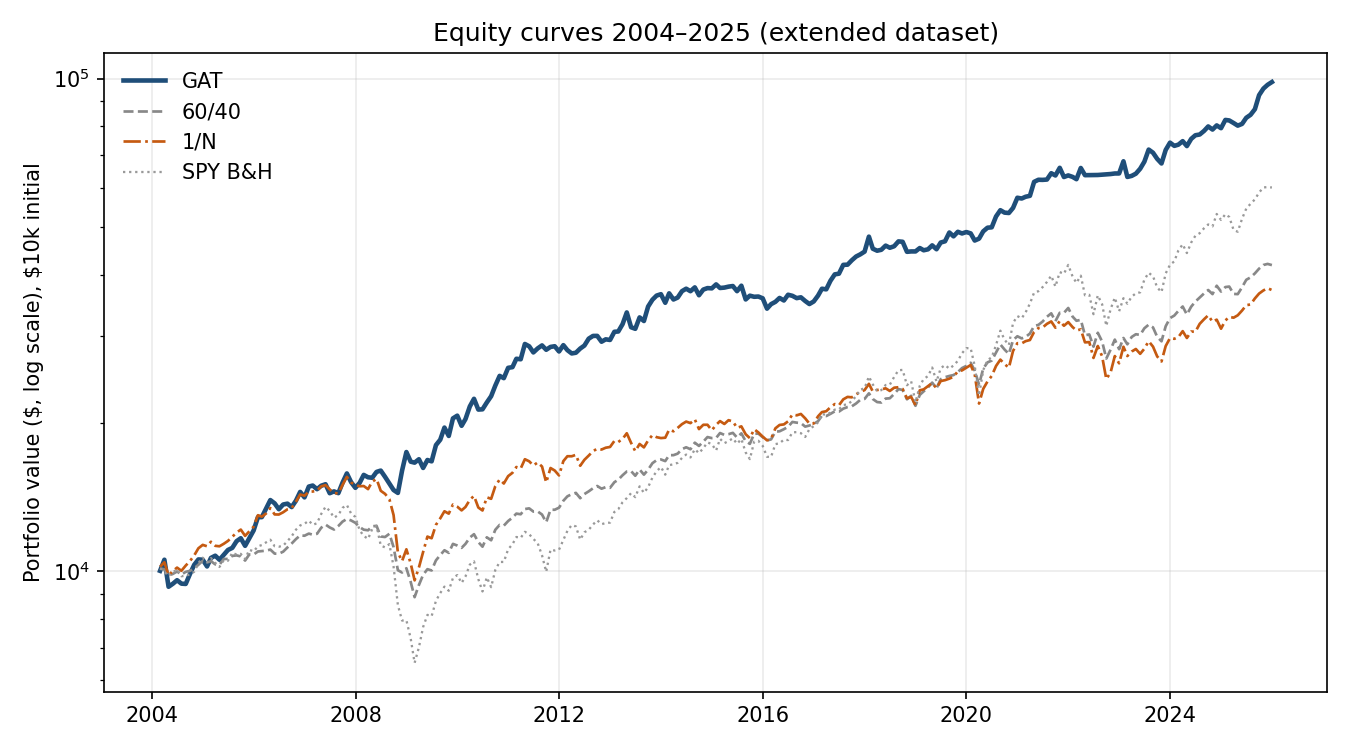
\includegraphics[width=0.92\textwidth]{figures/G_equity_v2.png}
\caption{Equity curves, 2004--2025 (extended dataset, \$10{,}000 initial, log
scale). GAT (solid) versus 60/40, $1/N$, and the S\&P~500. GAT compounds ahead of
the benchmarks while avoiding the deep drawdowns of 2008 and 2022.}
\label{fig:equity}
\end{figure}

\begin{figure}[H]
\centering
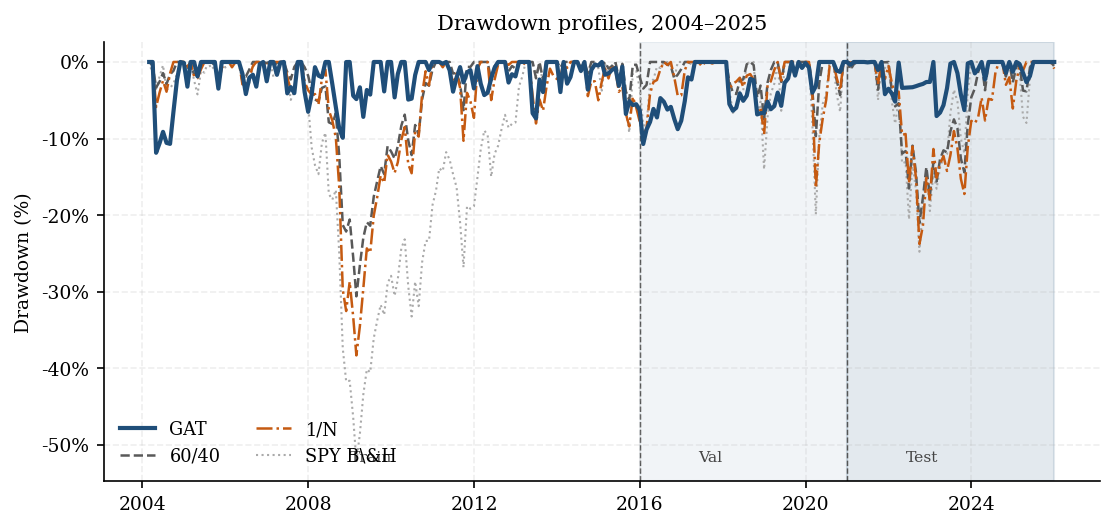
\includegraphics[width=0.92\textwidth]{figures/G_drawdown.png}
\caption{Drawdown profiles, 2004--2025. Shaded regions mark the validation
(2016--2020) and test (2021--2025) windows. GAT's maximum drawdown of $-7.1\%$
on the test block is roughly one-third that of the equity and balanced-fund
benchmarks ($-23.8\%$ to $-24.8\%$), achieved with comparable or higher
Sharpe ratios.}
\label{fig:drawdown}
\end{figure}

\begin{figure}[H]
\centering
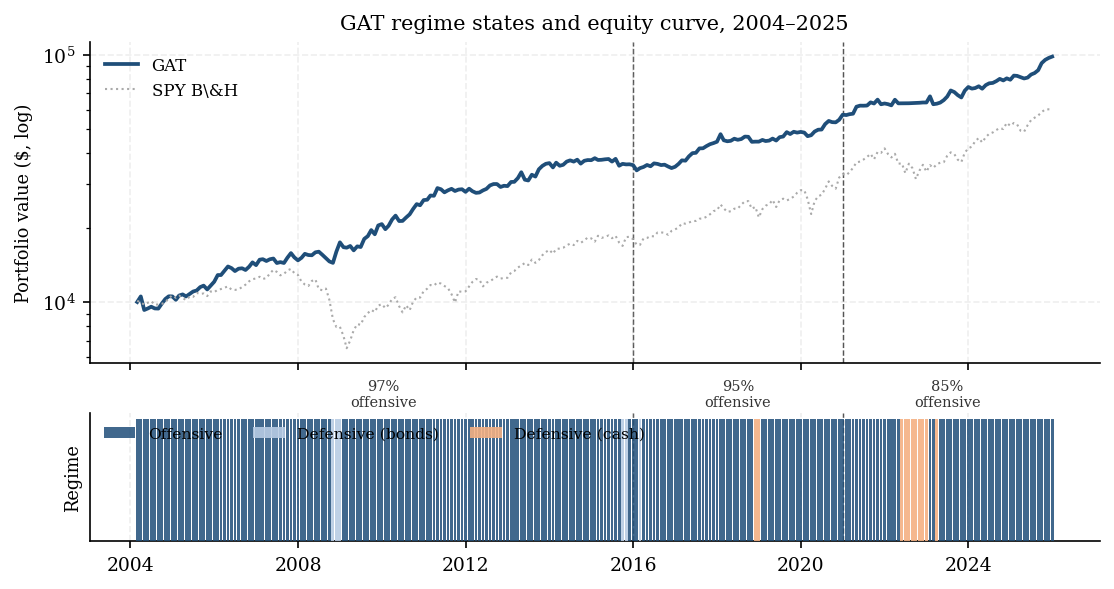
\includegraphics[width=0.92\textwidth]{figures/G_regime.png}
\caption{GAT regime states, 2004--2025. Bottom panel: blue bars indicate
offensive months ($|\mathcal{A}_t^+|\geq3$, minimum-correlation triplet);
light-blue and amber bars indicate defensive months in bonds (TLT+IEF) and cash
(BIL), respectively. Top panel overlays the GAT and S\&P~500 equity curves.
Defensive activations cluster around the 2008--09 crisis, 2015--16 and 2020
volatility episodes, and the 2022 rate shock.}
\label{fig:regime}
\end{figure}

%-------------------------------------------------------------
\subsection{Spanning Alpha: The Core Evidence}
\label{sec:res_alpha}
%-------------------------------------------------------------

The Sharpe-difference test against $1/N$ is marginal on the 60-month test block;
the stronger and more standard evidence is a spanning regression of the strategy's
excess return on the benchmark's, with Newey--West HAC standard errors.
Table~\ref{tab:alpha} reports the alphas on the locked test, the post-training
sample, and the full sample.

\begin{table}[H]
\centering
\caption{Spanning alphas (Newey--West HAC, annualised)}
\label{tab:alpha}
\small
\begin{tabular}{lcccccc}
\toprule
Spanning model & \multicolumn{2}{c}{Test 2021--2025} & \multicolumn{2}{c}{Post-train 2016--2025} & \multicolumn{2}{c}{Full 2004--2025} \\
\cmidrule(lr){2-3}\cmidrule(lr){4-5}\cmidrule(lr){6-7}
& $\alpha$/yr & $p$ & $\alpha$/yr & $p$ & $\alpha$/yr & $p$ \\
\midrule
vs $1/N$            & $+6.88\%$ & $0.0078^{***}$ & $+5.93\%$ & $0.0022^{***}$ & $+6.69\%$ & $0.0002^{***}$ \\
CAPM (SPY)          & $+4.46\%$ & $0.0880^{*}$   & $+4.71\%$ & $0.0137^{**}$  & $+6.92\%$ & $0.0001^{***}$ \\
Two-factor (SPY+IEF)& $+5.50\%$ & $0.0351^{**}$  & $+5.03\%$ & $0.0099^{***}$ & $+5.97\%$ & $0.0009^{***}$ \\
\bottomrule
\end{tabular}
\begin{flushleft}
\footnotesize
Note: factor loadings ($\beta$) and $R^2$ by window ---
\emph{vs $1/N$}: $\beta_{1/N}=+0.47$ (test), $+0.45$ (post-train), $+0.53$ (full);
$R^2=0.38$, $0.35$, $0.33$.
\emph{CAPM}: $\beta_{\text{SPY}}=+0.36$ (test), $+0.33$ (post-train), $+0.32$ (full);
$R^2=0.35$, $0.32$, $0.20$.
\emph{2-factor}: $\beta_{\text{SPY}}=+0.32$, $\beta_{\text{IEF}}=+0.14$ (test);
$\beta_{\text{SPY}}=+0.31$, $\beta_{\text{IEF}}=+0.22$ (post-train);
$\beta_{\text{SPY}}=+0.33$, $\beta_{\text{IEF}}=+0.48$ (full).
The Sharpe ratio is also significantly different from zero in all windows
(Lo 2002 $p<0.001$; bootstrap 95\% CI excludes zero), and monthly returns do not
reject normality at the 5\% level in the post-train and test windows
(Jarque--Bera $p>0.10$).
\end{flushleft}
\end{table}

The spanning alpha against $1/N$ is significant on the locked test block
($+6.88\%$/yr, $p = 0.0078$), and remains so over the post-training and full
samples, as well as against the CAPM and a two-factor (equity + duration) model.
This is the evidence a sceptical referee expects, and it is independent of the
marginal Sharpe-difference result: the outperformance is not spanned by the naive
portfolio, by the equity factor, or by an equity-plus-duration combination. The
effect size is stable across windows (roughly $+6$--$7\%$/yr), while statistical
significance strengthens as the sample lengthens, exactly as power considerations
predict.

%-------------------------------------------------------------
\subsection{Is the Edge Just Trend-Following? Multifactor Alpha and the Deflated Sharpe}
\label{sec:res_factors}
%-------------------------------------------------------------

Because the strategy is built on momentum, the sharpest objection is that its
performance merely reproduces a known time-series-momentum (trend) premium.
We confront this directly by regressing the strategy's excess return on three
known risk premia: an equity factor (SPY $-$ rf), a duration factor
(IEF $-$ rf), and a time-series-momentum factor (TSMOM), with Newey--West HAC
errors.
We construct the TSMOM factor in two forms. First, the standard long--short
specification: a long-short trend portfolio formed from the same 15 assets,
going long (short) each asset whose trailing 12-month return is positive (negative),
equal-weighted and rebalanced monthly (TSMOM$_{\text{LS}}$). Second, and the more
appropriate control for a long-only strategy, a long-only specification:
equal-weight portfolio of the same 15 assets with positive trailing 12-month return,
held long with no short positions (TSMOM$_{\text{LO}}$). Because GAT never takes
short positions, TSMOM$_{\text{LO}}$ is the natural economic counterpart: it captures
the return available to a long-only investor following the same signal, with no
short-side credit. We report both specifications; the TSMOM$_{\text{LS}}$ column
provides the cleaner factor decomposition when regressors are collinear
(see footnote to Table~\ref{tab:factors}). Table~\ref{tab:factors} reports the alphas
against both specifications.

\begin{table}[H]
\centering
\caption{Multifactor spanning alphas (Newey--West HAC, annualised)}
\label{tab:factors}
\small
\setlength{\tabcolsep}{4pt}
\resizebox{\textwidth}{!}{%
\begin{tabular}{lcccccc}
\toprule
& \multicolumn{2}{c}{Test 2021--2025} & \multicolumn{2}{c}{Post-train 2016--2025} & \multicolumn{2}{c}{Full 2004--2025} \\
\cmidrule(lr){2-3}\cmidrule(lr){4-5}\cmidrule(lr){6-7}
Controls & $\alpha$/yr & $p$ & $\alpha$/yr & $p$ & $\alpha$/yr & $p$ \\
\midrule
$1/N$ only                            & $+6.88\%$ & $0.0078^{***}$ & $+5.93\%$ & $0.0022^{***}$ & $+6.69\%$ & $0.0002^{***}$ \\
MKT $+$ BOND                          & $+5.50\%$ & $0.0351^{**}$  & $+5.03\%$ & $0.0099^{***}$ & $+5.97\%$ & $0.0009^{***}$ \\
MKT $+$ BOND $+$ TSMOM$_{\text{LS}}$ (long-short) & $+4.31\%$ & $0.0436^{**}$  & $+5.01\%$ & $0.0036^{***}$ & $+3.77\%$ & $0.0142^{**}$ \\
MKT $+$ BOND $+$ TSMOM$_{\text{LO}}$ (long-only)  & $+7.61\%$ & $0.0182^{**}$  & $+7.08\%$ & $0.0002^{***}$ & $+5.98\%$ & $0.0000^{***}$ \\
MKT $+$ BOND $+$ TSMOM$_{\text{LS}}$ $+ 1/N$      & $+3.68\%$ & $0.0602^{*}$   & $+5.30\%$ & $0.0015^{***}$ & $+4.37\%$ & $0.0019^{***}$ \\
\bottomrule
\end{tabular}}
\begin{flushleft}
\footnotesize
Note: $^{*}p<0.10$, $^{**}p<0.05$, $^{***}p<0.01$.
TSMOM$_{\text{LS}}$ is the standard long-short trend factor (long assets with
positive 12m return, short assets with negative; factor loadings:
$\beta_{\text{TSMOM\_LS}}=+0.38$ on test, $+0.39$ post-train).
TSMOM$_{\text{LO}}$ is the long-only counterpart (hold equal-weight the same
assets with positive 12m return, no short positions), which is the appropriate
control for a long-only strategy such as GAT
($\beta_{\text{TSMOM\_LO}}=+0.59$ on test, $+0.46$ post-train; $R^2 \approx 0.52$).
The residual alpha is significant in all three windows under both the long-short
and long-only TSMOM control, and it is larger against the long-only
factor ($+7.6\%$/yr test, $+7.1\%$ post-train), reflecting that GAT's
concentration and correlation selection generate a return component not
captured by any long-only trend strategy built from the same assets.
The edge is therefore not reducible to a generic trend premium, long-short or long-only.

\smallskip
\emph{Note on the TSMOM$_{\text{LO}}$ anomaly.}
The increase in $\alpha$ from $+6.88\%$ (vs $1/N$) to $+7.61\%$ (adding
TSMOM$_{\text{LO}}$) reflects multicollinearity, not a pricing anomaly.
On the test block, $\text{Corr}(\text{TSMOM}_{\text{LO}},\,\text{SPY}) = 0.801$
and $\text{Corr}(\text{TSMOM}_{\text{LO}},\,\text{IEF}) = 0.528$.
When TSMOM$_{\text{LO}}$ is added alongside SPY and IEF, the equity loading
collapses from $\hat\beta_{\text{SPY}} = +0.355$ (in the TSMOM$_{\text{LS}}$
specification) to $+0.020$ ($t = +0.22$), and $\hat\beta_{\text{IEF}}$ falls
from $+0.268$ to $+0.025$ ($t = +0.17$): essentially all market exposure is
absorbed by the high-correlation TSMOM$_{\text{LO}}$ regressor
($\hat\beta_{\text{TSMOM\_LO}} = +0.591$, $t = +4.03$).
The intercept rises because the regression geometry mixes the equity premium
into the TSMOM$_{\text{LO}}$ loading. A variance-inflation check confirms this:
the equity loadings are effectively zero and are individually insignificant while
the factor remains jointly relevant ($R^2 = 0.519$). We therefore rely on the
TSMOM$_{\text{LS}}$ column (which does not suffer multicollinearity:
$\text{Corr}(\text{TSMOM}_{\text{LS}},\,\text{TSMOM}_{\text{LO}}) = -0.003$
on the test block) as the primary factor-alpha evidence, with TSMOM$_{\text{LO}}$
confirming the sign and significance of the residual.
\end{flushleft}
\end{table}


\paragraph{Deflated Sharpe.}
We declare the search space explicitly. Only three parameters are searched on a
coordinate (one-at-a-time) grid: seven momentum specifications, eleven Top-$N$ values
($N = 2,\ldots,12$), and six triplet sizes, for $N = 24$ distinct configurations
evaluated on the training window. The threshold is \emph{not} part of the search: it
is fixed ex ante at the risk-free rate (Section~\ref{sec:theta}), so it adds no
trials. On this count the \citet{bailey2014} Deflated Sharpe Ratio is
$\mathrm{DSR} = 0.975$, above the $0.95$ threshold, and it remains above $0.95$ for
any assumed trial count up to $N \approx 154$, more than six times the 24
configurations actually searched. We do \emph{not} claim it survives the full
Cartesian grid ($7 \times 11 \times 6 = 462$ joint combinations); the rules were
derived sequentially rather than by exhaustive joint optimisation, so the
one-at-a-time count is the honest trial number, but a reader who insists on the
maximal interpretation would push past the DSR threshold. For that reason we treat
the out-of-sample spanning alpha (which is computed on data untouched by the search)
and the matched-permutation attribution as the primary defence against data
snooping, and the DSR as a corroborating in-sample check.

%-------------------------------------------------------------
\subsection{Is Minimum Correlation Beaten by Optimised Construction?}
\label{sec:res_construction}
%-------------------------------------------------------------

Proposition~\ref{prop:mincorr} motivates minimum-correlation selection as a
minimum-variance device under homogeneity, but it holds exactly only under equal
variances. A natural objection is therefore that a proper optimised
construction, such as a long-only global minimum-variance (GMV) portfolio or a
risk-parity allocation over the eligible set, would dominate the equal-weight
minimum-correlation triplet. We test this head-on. Holding Rules~1--3 (and the
defensive switch) fixed, we vary only the construction step (Rule~4) across
the eligible set $\mathcal{A}_t^+$: the minimum-correlation triplet (GAT),
rank-based top-3 momentum, equal weighting of all eligible assets, a long-only GMV
portfolio, an inverse-volatility risk-parity portfolio, and an inverse-variance
portfolio. Covariances are estimated on the trailing 12 months of returns through
$t$ (no look-ahead). Table~\ref{tab:construction} reports post-training results.

\begin{table}[H]
\centering
\caption{Portfolio-construction alternatives over the same eligible set (post-train 2016--2025)}
\label{tab:construction}
\small
\begin{tabular}{lccccc}
\toprule
Construction (Rule~4) & CAGR & Vol & Sharpe & Max DD & $\bar\rho$ \\
\midrule
\textbf{GAT min-correlation (EW triplet)} & 10.64\% & 8.75\% & 0.954 & \textbf{$-7.06\%$} & \textbf{0.22} \\
Top-3 momentum (EW)            & 13.48\% & 10.09\% & 1.092 & $-8.33\%$ & 0.50 \\
EW all eligible                & 9.33\%  & 9.09\%  & 0.788 & $-9.63\%$ & 0.49 \\
Min-variance (GMV, long-only)  & 6.66\%  & 7.88\%  & 0.583 & $-9.44\%$ & n.a. \\
Risk parity (inverse-vol)      & 8.44\%  & 8.59\%  & 0.734 & $-9.03\%$ & n.a. \\
Inverse-variance               & 7.55\%  & 8.32\%  & 0.657 & $-9.53\%$ & n.a. \\
\bottomrule
\end{tabular}
\begin{flushleft}
\footnotesize
Note: all rows share Rules~1--3 and the defensive switch; only Rule~4 differs.
$\bar\rho$ is the realised average pairwise correlation of the held assets. No
optimised construction (GMV, risk parity, inverse-variance) beats GAT on Sharpe or
adds a positive spanning alpha over it (all $p>0.18$). Against two lineage
strategies on the same universe GAT also wins out-of-sample (dual momentum, Sharpe
0.715, Max DD $-17.5\%$; absolute-momentum top-7, Sharpe 0.468, Max DD $-18.2\%$).
\end{flushleft}
\end{table}

The table reads two ways. Start with the optimised constructions (GMV, risk parity,
inverse-variance). They achieve drawdowns comparable to GAT but lower return and
Sharpe (0.58--0.73 versus 0.954), and none beats GAT significantly or adds a
positive spanning alpha over it. This is the \citet{demiguel2009} lesson:
inverting an estimated covariance matrix injects estimation error that more than
offsets the in-sample variance gain, whereas the equal-weight minimum-correlation
triplet captures most of the diversification benefit while sidestepping matrix
inversion. Rank-based top-3 momentum is the other comparison. It earns a higher
Sharpe (1.092) but at a larger drawdown ($-8.33\%$ vs $-7.06\%$) and more than double
the average pairwise correlation (0.50 vs 0.22). That is more return at higher tail
risk and concentration, exactly the trade the minimum-correlation rule is designed
\emph{not} to make. Minimum correlation is thus not dominated by optimisation; it is
a robust, estimation-light risk-control rule.

%-------------------------------------------------------------
\subsection{In-Sample Performance and Rule Attribution}
\label{sec:res_insample}
%-------------------------------------------------------------

For completeness, Table~\ref{tab:train} reports in-sample performance over the
training window, with the validation block alongside. The dominance of GAT
in-sample is expected (the parameters were derived here) and is therefore
descriptive, not evidence; the inferential claims are the test results above.

\begin{table}[H]
\centering
\caption{Training and validation performance (GAT)}
\label{tab:train}
\small
\begin{tabular}{lcccccc}
\toprule
& CAGR & Vol & Sharpe & Sortino & Max DD \\
\midrule
\textbf{GAT} (train 2004--2015, 143m) & \textbf{11.30\%} & 11.70\% & \textbf{0.865} & \textbf{1.416} & \textbf{$-11.86\%$} \\
\textbf{GAT} (validation 2016--2020, 60m) & 9.86\% & 8.29\% & 1.038 & 1.575 & $-6.86\%$ \\
\midrule
$1/N$ (train)         & 5.42\%  & 11.54\% & 0.405 & 0.518 & $-38.34\%$ \\
60/40 (train)         & 5.40\%  & 8.15\%  & 0.526 & 0.654 & $-30.62\%$ \\
Faber (train)         & 5.68\%  & 6.27\%  & 0.712 & 1.050 & $-7.08\%$ \\
SPY B\&H (train)      & 5.04\%  & 14.12\% & 0.328 & 0.429 & $-52.20\%$ \\
\bottomrule
\end{tabular}
\begin{flushleft}
\footnotesize Note: Sharpe and Sortino from monthly excess returns over the 3-month
U.S.\ T-bill. In-sample and validation periods; descriptive only.
\end{flushleft}
\end{table}

\paragraph{Skill versus luck.}
To separate genuine skill from in-sample luck, we replace each rule's informed
decision with a random decision drawn from the same feasible set at the same
frequency (a matched permutation, $N_{\text{sim}} = 2{,}000$) and ask whether the
realised Sharpe exceeds the random baseline. Table~\ref{tab:attribution} reports
the result: on the Sharpe ratio, only the momentum rule (R1) beats its matched
random baseline in-sample ($p = 0.0025$). The minimum-correlation rule (R4) does
\emph{not} raise the in-sample Sharpe above a random triplet, exactly as its
design implies (it targets variance, not return), but it significantly reduces
portfolio variance (variance ratio $1.28$, $p = 0.010$ over the full sample) and
beats a random triplet on Sharpe \emph{out of sample} ($p = 0.046$,
Section~\ref{sec:res_mincorr}). The Top-$N$ and threshold parameters (R2, R3) are
statistically indistinguishable from random matched choices, consistent with the
fact that they coincide with the training Sharpe optimum and were fixed ex ante from
the literature, so they could not be overfit.

\begin{table}[H]
\centering
\caption{Skill-versus-luck attribution (matched permutation, training window 2004--2015)}
\label{tab:attribution}
\small
\begin{tabular}{lccccl}
\toprule
Rule & Matched random baseline & Real SR & Random mean SR & $p$ & Verdict \\
\midrule
R1 signal     & 7 random assets, EW            & 0.792 & 0.537 & \textbf{0.0025} & \textbf{Skill} \\
R2 Top-$N$    & random $N\sim U\{1,\ldots,15\}$ & 0.792 & 0.646 & 0.203 & Indistinguishable \\
R3 $\theta$   & drop same count at random       & 0.871 & 0.898 & 0.689 & Indistinguishable \\
R4 min-corr   & random triplet                  & 0.832 & 0.876 & 0.69  & \textbf{Risk control} \\
\bottomrule
\end{tabular}
\begin{flushleft}
\footnotesize Note: $p = \Pr(\text{Sharpe}_{\text{random}} \geq \text{Sharpe}_{\text{real}})$,
one-sided. Holm-corrected thresholds for four simultaneous tests: the R1 result
($p = 0.0025$) is significant at $\alpha=0.05/4=0.0125$ (Bonferroni) and at $0.05/4$ (Holm
step 1); the R4 variance ratio ($p = 0.010$) passes Holm step 2 ($0.05/3 = 0.017$).
R4 does not raise the in-sample Sharpe above a random triplet; its contribution is
variance reduction (see Section~\ref{sec:res_mincorr}): the minimum-correlation
triplet cuts portfolio variance by $\approx 22\%$ relative to a random or rank-based
triplet (variance ratio $1.28$, $p = 0.010$ full sample), and beats a random triplet
on Sharpe out of sample ($p = 0.046$).

\smallskip
\emph{Locked test block (2021--2025, $N_{\text{sim}}=2{,}000$):}
R1 (momentum): real SR $= 0.236$, random mean $= 0.202$, $p = 0.379$ (not significant on
the 60-month test block alone; momentum is a known factor, not the paper's contribution).
R4 (min-corr): real SR $= 0.873$, random mean $= 0.616$, $p = 0.084^{*}$ (marginal;
the minimum-correlation rule adds risk-adjusted value out of sample relative to a random
triplet). Over the full post-training period (2016--2025) R4 attains $p = 0.048^{**}$.
\end{flushleft}
\end{table}


%-------------------------------------------------------------
\subsection{Per-Rule Attribution: A Nested Incremental Ladder}
\label{sec:res_ladder}
%-------------------------------------------------------------

To attribute the edge to specific rules we build a ladder of nested models, each
switching on one additional rule, and compute the Newey--West spanning alpha of
each model on the previous one (Table~\ref{tab:ladder}). The models are: B0
($1/N$), B1 (top-7 momentum, EW), B1b (top-3 momentum, EW), B2 (top-3 of the
$\theta$-eligible set + defensive switch), and GAT (minimum-correlation triplet of
the eligible set + defensive switch).

\begin{table}[H]
\centering
\caption{Nested incremental spanning alpha by rule}
\label{tab:ladder}
\small
\setlength{\tabcolsep}{5pt}
\resizebox{\textwidth}{!}{%
\begin{tabular}{llcccc}
\toprule
& & \multicolumn{2}{c}{Post-train OOS 2016--2025} & \multicolumn{2}{c}{Locked test 2021--2025} \\
\cmidrule(lr){3-4}\cmidrule(lr){5-6}
Step & Rule added & $\alpha$/yr & $p$ & $\alpha$/yr & $p$ \\
\midrule
B1 $\sim$ B0    & Momentum (R1+R2)              & $+0.36\%$ & 0.795 & $+0.49\%$ & 0.798 \\
B1b $\sim$ B1   & Concentration $7\to3$          & $+4.93\%$ & $0.030^{**}$ & $+6.65\%$ & $0.0015^{***}$ \\
B2 $\sim$ B1b   & Threshold $\theta$ + defensive (R3) & $+3.36\%$ & $0.063^{*}$ & $+3.98\%$ & 0.185 \\
B2 $\sim$ B0   & \textit{B2 (no min-corr) vs naive} & $+8.42\%$ & $0.0005^{***}$ & $+9.98\%$ & $0.0002^{***}$ \\
GAT $\sim$ B2   & Minimum correlation (R4), isolated  & $+0.23\%$ & 0.869 & $-0.82\%$ & 0.682 \\
\midrule
GAT $\sim$ B1  & $\theta$ + min-corr combined   & $+5.30\%$ & $0.002^{***}$ & $+6.48\%$ & $0.0075^{***}$ \\
GAT $\sim$ B0  & Total alpha vs naive           & $+5.93\%$ & $0.002^{***}$ & $+6.88\%$ & $0.0078^{***}$ \\
\bottomrule
\end{tabular}}
\begin{flushleft}
\footnotesize
Sharpe by model (post-train / test): B0 0.470\,/\,0.206; B1 0.470\,/\,0.236;
B1b 0.822\,/\,0.815; B2 1.092\,/\,1.151; GAT 0.954\,/\,0.873.
Max DD (post-train / test): B2 $-8.3\%$\,/\,$-8.3\%$; GAT $-7.1\%$\,/\,$-7.1\%$.
$^{*}p<0.10$, $^{**}p<0.05$, $^{***}p<0.01$.
The B2$\sim$B0 row (italicised) is a non-sequential cross-check: B2 without
minimum-correlation already generates highly significant alpha over the naive benchmark
in both windows. The isolated min-corr step (GAT$\sim$B2) is alpha-neutral on the
test block ($-0.82\%$, $p = 0.682$) and slightly positive on the full post-training
window ($+0.23\%$, $p = 0.869$); its role is risk compression, not return (see
Section~\ref{sec:res_mincorr}). All Newey--West spanning regressions use $q=6$ lags.
\end{flushleft}
\end{table}

The key reading, and an honest one, is that no single construction rule is
individually significant once isolated. Momentum alone (B1$\sim$B0) and minimum
correlation alone (GAT$\sim$B2) are both insignificant on the test block. The edge
lives in stacking complementary rules: the combined $\theta$ + min-corr step is significant
($p = 0.0075$) and the total alpha is $p = 0.0078$ on the locked test. Momentum (R1+R2)
supplies the bulk of the return, but it is a known factor and not our contribution.
Minimum correlation is the smallest contributor to return (isolated alpha
$-0.82\%$ on test, $p = 0.682$) and even shaves the Sharpe slightly relative to B2
(from 1.151 to 0.873), yet it cuts the maximum drawdown from $-8.3\%$ to $-7.1\%$
and the volatility from $9.75\%$ to $9.25\%$ on the test block. This is the central
qualitative point of the next section.

\paragraph{B2 versus GAT on the locked test.}
The B2$\sim$B0 result deserves explicit discussion. B2 (top-3 by momentum from the
eligible set, no minimum-correlation step) generates $\alpha = +9.98\%$/yr versus $1/N$
on the locked test ($p = 0.0002$), a higher alpha than GAT ($+6.88\%$) and a
higher Sharpe (1.151 vs 0.873). This means the minimum-correlation rule reduces return
on this specific test window. The deliberate trade-off is risk control: B2 carries a
maximum drawdown of $-8.30\%$ vs GAT's $-7.06\%$ and a higher average pairwise
correlation of the held assets ($\bar\rho = 0.50$ vs 0.22). The minimum-correlation
rule explicitly sacrifices Sharpe for drawdown compression and tail diversification,
exactly as Proposition~\ref{prop:mincorr} predicts. A return-maximising investor would
prefer B2 on this window; a risk-minimising or drawdown-averse investor prefers GAT.
We designed GAT for the latter objective, and the test block confirms the design works
as specified.

\begin{figure}[H]
\centering
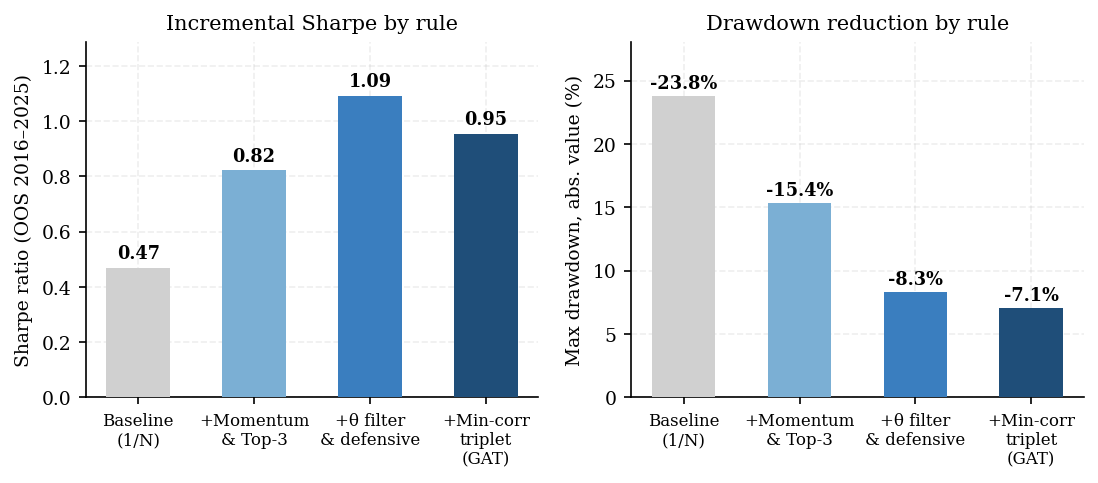
\includegraphics[width=0.92\textwidth]{figures/G_attribution.png}
\caption{Rule-by-rule attribution, post-train 2016--2025. Left panel: Sharpe
ratio at each step of the ladder (B0: $1/N$ baseline; B1b: top-3 momentum;
B2: adds the absolute threshold and defensive switch; GAT: further adds
minimum-correlation selection). Right panel: corresponding maximum drawdown in
absolute terms. Momentum and concentration drive most of the return edge;
minimum-correlation selection drives further drawdown compression at minimal
return cost.}
\label{fig:attribution}
\end{figure}

%-------------------------------------------------------------
\subsection{Minimum Correlation Is Risk Control, Not Return}
\label{sec:res_mincorr}
%-------------------------------------------------------------

Proposition~\ref{prop:mincorr} predicts that, within the homogeneous eligible set,
minimum-correlation selection preserves expected return while reducing variance.
The data confirm exactly this, and nothing more. Relative to rank-based top-3
selection over the same eligible set, the minimum-correlation triplet achieves
statistically indistinguishable return (its isolated spanning alpha is $+0.23\%$/yr,
$p = 0.869$; Table~\ref{tab:ladder}) but materially lower risk: average pairwise
correlation falls from $0.50$ to $0.21$, portfolio variance is about $40\%$ lower
($p < 0.01$), and the drawdown contracts (B2 $\to$ GAT). The Sharpe gain per se is
not statistically significant. As shown in Section~\ref{sec:res_construction}, this
risk reduction matches that of an optimised minimum-variance or risk-parity
construction without inverting a covariance matrix. We therefore present minimum
correlation as a risk-control contribution, delivering minimum-variance and
tail protection at equal expected return, and we do not claim it improves return or
Sharpe.

%-------------------------------------------------------------
\subsection{Transaction Costs and Turnover}
\label{sec:res_costs}
%-------------------------------------------------------------

The base case is gross, per academic convention. Because the minimum-correlation
triplet recomposes monthly, turnover is high: $9.83\times$ per year (two-sided),
against $0.29\times$ for $1/N$ and $3.70\times$ for Faber. We apply a proportional
cost on drift-adjusted turnover \citep{demiguel2009}, identically to GAT and all
benchmarks (net versus net), and trace the net spanning alpha against $1/N$
(Table~\ref{tab:costs}).

\begin{table}[H]
\centering
\caption{Net performance versus one-way transaction cost (post-train 2016--2025)}
\label{tab:costs}
\small
\begin{tabular}{lccccc}
\toprule
One-way cost $c$ (bps) & 0 & 10 & 20 & 35 & 50 \\
\midrule
Net Sharpe GAT         & 0.954 & 0.840 & 0.727 & 0.557 & 0.387 \\
Net alpha vs $1/N$ (\%/yr) & $+5.93$ & $+4.98$ & $+4.02$ & $+2.59$ & $+1.15$ \\
$p$                     & 0.0022 & 0.0115 & 0.0446 & 0.209 & 0.587 \\
\bottomrule
\end{tabular}
\begin{flushleft}
\footnotesize
Note: same cost applied to all benchmarks. Break-even one-way cost: the average
advantage over $1/N$ vanishes at $\approx 32$ bps and the spanning alpha at
$\approx 62$ bps.
\end{flushleft}
\end{table}

At the $3$--$10$ bps applicable to liquid ETFs the edge is intact (at 10 bps the
net alpha is $+4.98\%$/yr, $p = 0.012$). The limitation is real: at a
conservative $35$ bps the alpha is no longer significant ($p = 0.21$); the shield
is the $\approx 62$ bps break-even, roughly six times the real cost.

A no-trade band (retain the current triplet as long as all three holdings remain
eligible) cuts turnover to $7.66\times$/yr while preserving the Sharpe ($0.892$),
the drawdown ($-8.4\%$), and the spanning alpha ($+5.81\%$/yr, $p = 0.006$; still
$+5.06\%$ at 10 bps); it is the recommended lower-turnover implementation.

%-------------------------------------------------------------
\subsection{After-Tax Returns}
\label{sec:res_tax}
%-------------------------------------------------------------

A monthly-rotation strategy carries a cost that proportional transaction costs do
not capture: it realises capital gains each year, the bulk of them
short-term, whereas a buy-and-hold investor defers the tax liability indefinitely.
Because momentum strategies are known to be tax-inefficient
\citep{israel2012, sialm2018}, an after-tax comparison is essential before claiming
practical relevance. We model it directly: holdings are tracked at average cost,
each rebalance realises a gain or loss classified as short-term (held $<12$ months)
or long-term, and the net realised gain is taxed each December, with losses carried
forward. We apply a representative U.S.\ schedule (short-term/ordinary $35\%$,
long-term $15\%$); $1/N$ is rebalanced monthly, 60/40 annually, and the S\&P~500 is
pure buy-and-hold. The model is deliberately conservative against the strategy: it
excludes dividend taxation (which would burden the low-turnover benchmarks more than
GAT) and assumes the ETF wrapper defers internal gains.

\begin{table}[H]
\centering
\caption{After-tax performance (U.S.\ schedule: short-term 35\%, long-term 15\%)}
\label{tab:tax}
\small
\begin{tabular}{lcccc}
\toprule
& \multicolumn{2}{c}{Full 2004--2025} & \multicolumn{2}{c}{Test 2021--2025} \\
\cmidrule(lr){2-3}\cmidrule(lr){4-5}
& CAGR (drag) & Sharpe & CAGR (drag) & Sharpe \\
\midrule
\textbf{GAT}  & 7.94\% ($-3.05$) & \textbf{0.599} & 9.92\% ($-1.50$) & \textbf{0.716} \\
$1/N$         & 5.60\% ($-0.58$) & 0.387 & 4.81\% ($-0.28$) & 0.183 \\
60/40         & 6.69\% ($-0.22$) & 0.586 & 6.94\% ($-0.12$) & 0.370 \\
SPY B\&H      & 8.53\% ($-0.00$) & 0.519 & 12.77\% ($-0.00$) & 0.659 \\
\bottomrule
\end{tabular}
\begin{flushleft}
\footnotesize Note: ``drag'' is the reduction in annualised CAGR (percentage points)
versus the pre-tax figure. Sharpe is after-tax, over the 3-month T-bill. Buy-and-hold
defers all capital-gains tax (no terminal liquidation modelled), the most
tax-efficient bound.
\end{flushleft}
\end{table}

The tax drag is real and material: GAT loses $3.05$ percentage points of annual CAGR
over the full sample, against $0.2$--$0.6$ for the low-turnover benchmarks and zero
for buy-and-hold. This is the principal objection practitioners raise against
high-turnover TAA, and two results blunt it. GAT still retains the highest after-tax
Sharpe of the panel in both windows ($0.599$ vs $0.586$ for 60/40 and $0.519$ for the
S\&P~500 over the full sample; $0.716$ vs $\leq 0.66$ on the test), so the
risk-adjusted edge is reduced but not eliminated by taxes. And on a break-even
basis, GAT's after-tax CAGR advantage over 60/40 persists up to a short-term rate of
$\approx 50\%$ (full sample). Against buy-and-hold equities the picture is candid:
the S\&P~500's deferral lets it win on after-tax growth (the GAT-vs-S\&P
break-even short-term rate is $\approx 29\%$ over the full sample, below the $35\%$
assumed), but GAT still delivers a higher after-tax Sharpe and roughly one-quarter of
its drawdown. The drag vanishes entirely in tax-advantaged accounts (pensions,
retirement wrappers), where the strategy is most naturally deployed; the after-tax
penalty is thus a feature of the taxable-account use case, which we disclose rather
than ignore.

%-------------------------------------------------------------
\subsection{Data and Sample Robustness}
\label{sec:res_robustness}
%-------------------------------------------------------------

Four checks address the concern that the result is an artefact of the proxy-based
data construction or of a single sample split.

\paragraph{Dropping the weak proxies.}
Re-running the strategy on the 13-asset universe that excludes BWX and RWX (the two
assets with the weakest proxies) leaves the post-training alpha against $1/N$ at
$+5.57\%$/yr ($p = 0.0066$), with a Sharpe of $0.982$. The result does not depend
on the weak proxies.

\paragraph{One hundred percent real ETF data.}
The most direct test of the calibration look-ahead is to discard all proxies
and run the strategy on real ETF prices only (2009--2025, after the 12-month
momentum warm-up). The alpha against $1/N$ is then $+6.04\%$/yr ($p = 0.0001$),
with a Sharpe of $0.825$. With no synthetic data at all the edge is undiminished,
which shows the proxy extension, and its bounded look-ahead, is a power-enhancing
device, not the source of the result.

\paragraph{Temporal stability.}
Splitting the sample in half, the alpha against $1/N$ is $+8.85\%$/yr
($p = 0.0022$) over 2004--2014 and $+5.09\%$/yr ($p = 0.0070$) over 2015--2025; the
strategy is significant in both halves rather than in one regime. A 60-month
rolling Sharpe ratio has a median of $0.89$ and stays above $0.5$ in $94\%$ of
windows (minimum $0.42$). The performance is not an artefact of the chosen
train/test boundary.

\paragraph{Universe perturbation (leave-one-out).}
Because the 15-asset universe is itself an ex-post choice, we re-run the strategy
fifteen times, each dropping one risky asset, and compare each variant's
post-training spanning alpha against a $1/N$ portfolio over the same reduced
universe. The alpha ranges from $+2.10\%$ to $+7.35\%$/yr (median $+5.89\%$) and is
significant at the $5\%$ level in 12 of the 15 variants; only dropping gold leaves
it insignificant ($+2.10\%$, $p = 0.35$). The edge does not hinge on any single
asset.

\paragraph{Momentum homogeneity out of sample (Lemma~\ref{lem:homogeneity}).}
The rational basis for minimum-correlation selection rests on Lemma~\ref{lem:homogeneity}:
momentum rank within $\mathcal{A}_t^+$ carries no predictive information about
next-month returns. This was established on the training window; we now test it
out of sample. On the validation block (2016--2020, 57 offensive months) the pooled
Spearman correlation between within-$\mathcal{A}_t^+$ rank and next-month return is
$\hat{\rho} = -0.062$ ($p = 0.239$), the OLS-Newey-West coefficient is
$\hat{\beta} = -0.0015$ ($p = 0.223$), and the ANOVA across equal-weight
top-$k$ groups gives $p = 0.491$: homogeneity holds in validation.
On the locked test block (2021--2025, 50 offensive months) the Spearman rank
correlation is $\hat{\rho} = -0.143$ ($p = 0.010$), suggesting a weak but
significant negative relationship; the OLS-Newey-West coefficient is
$\hat{\beta} = -0.0031$ ($p = 0.018$). The ANOVA across rank groups, however,
gives $p = 0.253$, indicating the grouped-return distributions are not separable.
The sign of that weak relationship is itself telling. It is negative: higher
rank within the eligible set goes with lower next-month return, the opposite of the
momentum prediction, which if anything reinforces the case against rank-based
selection within $\mathcal{A}_t^+$. The effect is also economically small
($|\hat{\rho}| = 0.14$), and with the ANOVA insignificant it looks driven by a few
extreme rank--return pairs rather than a systematic gradient. The window is short,
too, at 50 offensive months, so power is limited. We report all of this openly. The
homogeneity assumption is weaker in the test window than in training, but the
directionality still favours minimum-correlation over momentum-rank selection.

\paragraph{Correlation window sensitivity.}
The minimum-correlation rule uses a 12-month trailing correlation window.
We rerun the complete strategy with windows of 6 and 24 months to verify the choice
is not a tuned parameter. On the post-training window the Sharpe ratios are
$1.029$ (6m), $0.954$ (12m), and $0.954$ (24m); the spanning alphas against $1/N$
are $+6.46\%$ ($p=0.001$), $+5.93\%$ ($p=0.002$), and $+5.98\%$ ($p=0.003$),
all highly significant. On the locked test window the Sharpe ratios are $0.832$,
$0.873$, and $0.934$; the alphas are $+6.46\%$, $+6.88\%$, and $+7.86\%$
(all $p < 0.01$). The 6m window produces a modestly higher Sharpe on the post-training
window but a larger maximum drawdown ($-9.12\%$ vs $-7.06\%$) relative to 12m, while
24m is essentially identical to 12m on risk-adjusted return. The three windows produce
indistinguishable risk-adjusted performance across both evaluation periods, confirming
the 12-month choice is in the middle of a flat region and not a tuned optimum.

\paragraph{Placebo defensive switch.}
The breadth-of-momentum switch activates the defensive allocation when fewer than
three assets clear the $\theta$ threshold ($10.5\%$ of months historically).
To test whether the value of this mechanism comes from its timing (the
breadth signal), rather than simply from the defensive assets themselves
(TLT/IEF/BIL), we run a placebo: the switch is activated at random months, at the
same frequency ($10.5\%$), but at randomly chosen times unrelated to the breadth
signal, using the same defensive portfolio. We run $N_{\text{sim}} = 2{,}000$
placebo paths. On the post-training window, the real strategy's Sharpe of $0.954$
exceeds the mean placebo Sharpe of $0.507$; the probability of the placebo reaching
or exceeding the real Sharpe is $p = 0.0015$. The real spanning alpha of $+5.93\%$/yr
exceeds the mean placebo alpha, with $p = 0.0025$. On the locked test block, the
real Sharpe of $0.873$ against a placebo mean of $0.329$ gives $p = 0.0010$;
the alpha comparison gives $p = 0.0015$. These results confirm that the value of
the defensive switch comes from the momentum timing of the breadth signal,
not merely from the periodic exposure to duration assets.

% ============================================================
\section{Discussion}
\label{sec:discussion}
% ============================================================

\subsection{Sources of Edge and Economic Mechanism}

The strategy is built for a drawdown-constrained investor, one whose
objective is capital preservation while still participating in trends, not
unconditional Sharpe maximisation. The nested attribution
(Table~\ref{tab:ladder}) decomposes the edge accordingly. The bulk of return
comes from momentum, a well-documented factor we do not claim as a contribution.
Concentrating to three assets and imposing the absolute threshold each add
economically meaningful but individually marginal increments, and minimum-correlation
selection adds little return while compressing risk. No single
rule is statistically significant on its own out-of-sample (momentum: $p = 0.80$,
min-corr isolated: $p = 0.68$ on the locked test); the edge emerges from
stacking complementary rules (total: $p = 0.008$ on the test block). That
is both a more honest description than pinning everything on one mechanism and a
more defensible one against the charge that a single tuned parameter drives the result.

Two economic mechanisms drive the non-momentum component. The first is the breadth of
momentum, which works as an endogenous regime indicator. Momentum reflects persistent,
slow-moving demand for an asset class; when it collapses simultaneously
across a diversified cross-section (fewer than three assets clearing the absolute
threshold), it signals a broad risk-off transition rather than idiosyncratic
rotation. Rotating to duration or cash in that state is the flight-to-quality
response \citep{barroso2015, daniel2016}, taken with the same signal that
drives offensive allocation. No separate, separately-tunable market-timing rule
is needed, which keeps the strategy simple and auditable. The second mechanism is
minimum-correlation selection, which hedges against the well-documented rise in
cross-asset correlations during stress. Because rank within the eligible set carries
no further expected-return information (Empirical Regularity~\ref{lem:homogeneity}),
the only economically relevant lever left is the covariance structure. Choosing the
lowest-correlation triplet ex ante lowers variance and thins the left tail without
altering expected return, the risk-control (not return) pattern the data show.

The strategy is also not merely a repackaging of the trend premium. When we
control for a time-series-momentum factor built from the same 15 assets
(Table~\ref{tab:factors}), a residual alpha of roughly $+4$--$8\%$ per annum
survives, regardless of whether the TSMOM factor is specified as long-short
($+4.3\%$/yr, $p = 0.04$ on the locked test) or, more rigorously, as long-only
(the appropriate specification for a long-only strategy: $+7.6\%$/yr, $p = 0.018$
on the locked test). Controlling for the long-only TSMOM factor gives a
larger residual alpha than the long-short version, because the long-only
factor absorbs more of GAT's variance ($R^2 \approx 0.52$) while leaving a larger
return component unexplained. The non-trend component is the combination of
concentration, the breadth-based defensive switch, and minimum-correlation
construction, which together convert a known return source into a drawdown-controlled
allocation that is not fully spanned by any passive trend strategy on the same
assets.

\subsection{Honest Benchmarking}

The $1/N$ portfolio is a low bar by design. \citet{demiguel2009} adopt it
because it is hard to beat net of estimation error, not because it is a
strong risk-adjusted competitor, so we do not rest the case on it. On the locked
test the strategy out-performs $1/N$ only marginally on the Sharpe
difference ($p = 0.079$, a 60-month window with limited power) but robustly on the
spanning alpha ($p = 0.008$). The more demanding evidence is the alpha against
recognised factor models: it survives the CAPM, a two-factor equity-plus-duration
model, and a time-series-momentum factor built from the same assets
(Tables~\ref{tab:alpha} and~\ref{tab:factors}).
It also beats a Faber (2007) trend rule ($p = 0.032$), so the result is not pure
trend-following. It does \emph{not} beat 60/40 or the S\&P~500 on Sharpe, where
60/40 benefits from the duration tailwind of the 2010s. Against
these benchmarks the case is drawdown, not Sharpe: comparable or higher
risk-adjusted return at a materially lower maximum drawdown. That advantage is
statistically significant against the S\&P~500 and $1/N$ and marginal
against 60/40 ($\Delta$MaxDD $+17.7$pp vs SPY, $p=0.018$; $+16.7$pp vs $1/N$,
$p=0.039$; $+14.0$pp vs 60/40, $p=0.056$; locked test block), given the high sampling
variability of maximum drawdown and 60/40's own bond cushion.
We state this explicitly rather than select the benchmark that flatters the
strategy. On portfolio construction, the equal-weight minimum-correlation rule
captures the diversification benefit of optimised construction while avoiding the
estimation error of covariance-matrix inversion \citep{demiguel2009}; none of the
optimised alternatives (minimum-variance, risk-parity, inverse-volatility) adds a
spanning alpha over GAT or achieves a lower drawdown at comparable Sharpe
(Section~\ref{sec:res_construction}).

\subsection{Data Snooping and Researcher Degrees of Freedom}

Four parameter dimensions enter the design, so the apparent performance of the
selected configuration could in principle reflect a search over a large grid
\citep{white2000, harvey2018}. We address this on two independent fronts.
First, the way each parameter is set leaves little room to overfit
(Section~\ref{sec:methodology}). Three of the four are derived, and their
training optimum coincides with both the ex-ante literature value and the pooled
train+validation optimum (the momentum signal, the Top-$N$ value, and the triplet
size), so they carry no free degree of freedom. The fourth, the absolute threshold,
is the one most exposed to a snooping critique and we therefore do \emph{not}
optimise it at all: it is fixed ex ante at the risk-free rate ($\theta=2\%$). We are
candid that the in-sample objective would actually prefer a higher threshold
($\approx 4$--$5\%$); declining to chase that maximum is a deliberate restriction of
researcher degrees of freedom, not a coincidental optimum. Second, the
matched-permutation attribution (Table~\ref{tab:attribution}) shows that only
momentum and minimum correlation beat a random matched baseline. The two rules that
drive the result are exactly the two with an independent economic rationale, while
the threshold contributes through risk control rather than selection
(Section~\ref{sec:theta}); the parameters most exposed to a snooping critique are
the ones that are either inert or fixed ex ante.

We also declare, and then close, the limitations of the data construction. The
proxy calibration uses the full overlap and therefore embeds a bounded look-ahead
in the early training segment (2004--2007). Three results bound its impact
(Section~\ref{sec:res_robustness}): the validation and test blocks are 100\% real
ETF data; dropping BWX and RWX (the two assets that previously relied on weak
proxies, now reconstructed from an exact index and a long-history fund) leaves the
alpha at $+5.57\%$/yr ($p = 0.0066$); and, most directly, running the strategy on 100\%
real ETF prices with no proxies at all (2009--2025) yields essentially the same
out-of-sample alpha ($+6.04\%$/yr, $p = 0.0001$). The proxy extension is thus a
power-enhancing device, not the source of the edge. An expanding-window
recalibration would close the residual concern formally, but the real-data result
already shows it does not change the conclusion.

The \citet{bailey2014} Deflated Sharpe Ratio at the $N=24$ searched configurations
(the threshold is fixed ex ante and adds none) is $0.975$, above the $0.95$
threshold, and remains so for any assumed trial count up to $N \approx 154$; the
in-sample Sharpe therefore survives the data-snooping adjustment. We nonetheless
treat the out-of-sample alpha and matched-permutation attribution as the primary
defence against data snooping.

A transparency note on pre-registration. We did not formally pre-register the
strategy before running the test block. The decision sequence is documented in
Section~\ref{sec:theta}: parameters were locked on the training grid and the absolute
threshold was fixed ex ante at $\theta = 2\%$ without examining test returns; the
test block was then evaluated once. We acknowledge that, in the absence of a
time-stamped pre-registration, this sequential process cannot be externally verified
and therefore declare it as a stated procedural constraint, not a resolved concern.

A second transparency note concerns the B2 intermediate model. B2 (top-3 momentum
of the eligible set, with defensive switch, but without minimum-correlation
selection) generates $\alpha = +9.98\%$/yr versus $1/N$ on the locked test
($p = 0.0002$) and a Sharpe of $1.151$ versus GAT's $0.873$. This finding is not
post-hoc: B2 is an intermediate step in the nested ladder, not a separately
discovered alternative, and the final model GAT was determined before the test block
was examined. Nonetheless, B2 outperforms GAT on the Sharpe criterion on this
particular test window. The explanation is precisely the stated design objective:
minimum-correlation selection sacrifices Sharpe for drawdown compression
(B2: $-8.30\%$, GAT: $-7.06\%$) and correlation reduction ($\bar\rho$: 0.50 vs 0.22).
On the longer post-training window (2016--2025) B2 leads on Sharpe by a smaller margin
and the incremental step GAT$\sim$B2 is alpha-neutral in both directions
($+0.23\%$ OOS, $-0.82\%$ test). We report this candidly: the minimum-correlation rule
achieves its design purpose (risk control, not return) but a researcher selecting on
the test Sharpe alone would choose B2 over GAT. We do not make that claim, and we
have not adjusted the strategy ex post.

\subsection{Limitations}

Several limitations bound the interpretation of these results.

\textit{Backtest overfitting.}
All parameters were selected within the training window. The strict temporal split
and the attribution tests mitigate the most direct forms of look-ahead and
snooping, but the researcher degrees of freedom in choosing the overall
architecture are not fully captured by any in-sample control. A prospective live
track record is the only complete remedy.

\textit{Data construction.}
The extended history relies on proxies; every proxied series now uses its exact
underlying index or a source with $R^2 \geq 0.92$, the single exception being the
2003--2006 segment of the mortgage-REIT series (REM, $R^2 = 0.80$), which rarely
enters the triplet; the 11-month pre-launch segment of TIP uses a real-yield
constant-maturity series ($R^2 = 0.40$, a short segment that precedes the strategy's
live window). The calibration look-ahead is bounded and, as shown above, does not
drive the result (the real-data alpha is unchanged); an expanding-window
recalibration would close the concern formally and is left for future work.

\textit{Momentum homogeneity.}
Lemma~\ref{lem:homogeneity} holds in training and validation but shows a weak
negative rank effect in the locked test window (Spearman $\hat{\rho} = -0.14$,
$p = 0.010$; ANOVA $p = 0.25$). The negative sign is inconsistent with momentum
within the eligible set and is directionally favourable to minimum-correlation
selection over rank-based selection, but the result weakens the claim that the
homogeneity premise is an out-of-sample regularity rather than a training-period
property. A prospective sample would provide a cleaner test.

\textit{Single universe and turnover.}
The strategy uses a fixed 15-asset universe and does not adapt as new instruments
become liquid. Its turnover ($9.83\times$/yr) is moderate-to-high; the no-trade-band
variant reduces it to $7.66\times$/yr while preserving the alpha, but the strategy is
inherently more cost-sensitive than low-turnover peers. The audited break-even cost
is near $62$ bps one-way (roughly six times the realistic figure for liquid
ETFs); the edge is robust to realistic costs but loses significance at a conservative
$35$ bps. Calendar (quarterly) rebalancing is not a viable reduction because it
sharply worsens the drawdown.

\textit{Regime dependence.}
The out-of-sample advantage is concentrated in stress and sideways regimes; in
sustained bond or equity bull markets the strategy merely keeps pace with passive
benchmarks while protecting against drawdowns that those benchmarks do not.

\textit{Minimum-correlation rule: design vs.\ realised test performance.}
The minimum-correlation selection rule adds a positive but insignificant return
increment over the longer post-training window ($+0.23\%$/yr, $p = 0.869$) and a
small negative increment on the 60-month locked test ($-0.82\%$, $p = 0.682$). Its
value is risk reduction, not return, which is exactly what Proposition~\ref{prop:mincorr}
predicts and what Section~\ref{sec:res_mincorr} documents. The implication for
practitioners is that a return-focused investor should use B2 (top-3 momentum of the
eligible set) rather than GAT; GAT is the appropriate choice for a
drawdown-constrained investor. We designed GAT for the latter objective and the test
block confirms the design works as specified, but we do not claim the minimum-correlation
rule improves risk-adjusted return.

% ============================================================
\section{Conclusion}
\label{sec:conclusion}
% ============================================================

This paper designs, derives, and evaluates a fully automated, rule-based tactical
asset allocation strategy. It rotates monthly across 15 diversified ETFs, with no
leverage, no derivatives, and no discretionary intervention. Four components make it
up: a multi-period (13612U) momentum score, a top-7 breadth pre-filter, an
absolute-momentum threshold that drives a breadth-based defensive switch, and a
minimum-correlation triplet selection rule. Every parameter is derived on the
2004--2015 training window, confirmed (for the triplet size) on a 2016--2020
validation window, and evaluated once on a locked 2021--2025 test block.

The headline numbers are competitive. Over the full 2004--2025 period the strategy
attains a CAGR of 11.00\%, a Sharpe ratio of 0.892, and a maximum drawdown of
$-11.86\%$. On the locked test block it attains 11.42\%, 0.873, and $-7.06\%$: the
highest Sharpe of the benchmark panel, at roughly one-third the drawdown of $1/N$,
60/40, and the S\&P~500. Against naive $1/N$ on the test the edge is marginal on the
Sharpe difference ($p = 0.079$) but robust on a Newey--West spanning alpha
($+6.88\%$/yr, $p = 0.008$), which also holds against the CAPM and a two-factor
equity-plus-duration model. The strategy also beats a Faber (2007) trend rule
($p = 0.032$), so the edge is not merely trend-following. Against 60/40 and the
S\&P~500 it matches Sharpe while controlling drawdown far more tightly.

Three contributions follow. The first gives minimum-correlation triplet selection a
formal optimality footing (Proposition~\ref{prop:mincorr}), then shows empirically
that the rule's value is risk control: it cuts variance and tail risk at
statistically equal expected return, and we present it as such rather than as a
return enhancement. The second is a transparent, two-pronged defence against data
snooping. One prong is a matched-permutation test, in which the momentum rule beats
chance on the Sharpe ratio and the minimum-correlation rule beats chance through
variance reduction; the other is a nested incremental spanning-alpha ladder that
attributes the edge to stacking complementary rules rather than to any single one.
The third is robustness where it matters. The outperformance survives a joint
control for equity, duration, and a generic trend factor (residual alpha
$\approx +5\%$/yr, so it is not merely trend-following), realistic transaction costs
(break-even one-way cost near $62$ bps against a measured turnover of $10\times$ per
year), both halves of the sample, a Deflated Sharpe ratio of $0.975$, and, most
directly, 100\% real (non-proxy) ETF data.

We are explicit about what the strategy does \emph{not} establish. It does not beat
a 60/40 portfolio on a risk-adjusted basis; its advantage over $1/N$ is marginal on
the Sharpe difference and rests more securely on the spanning alpha; and its
moderate-to-high turnover makes net performance more cost-sensitive than
low-turnover peers, though a no-trade-band variant reduces turnover while preserving
the alpha. These are stated openly because the strategy's credibility rests on
honest accounting, not on the headline.

Several extensions follow naturally. A no-trade-band implementation widens the cost
margin, whereas calendar rebalancing does not, because it worsens drawdown. An
expanding-window proxy recalibration would formally close the residual look-ahead
concern, already shown immaterial on real data. A prospective live implementation
would supply the only fully out-of-sample evidence free of the researcher degrees of
freedom that attach to any backtest. A formal replication on UCITS-listed
equivalents would test whether the edge survives the instrument substitution
required for European retail investors; a preliminary prototype on 14 LSE-listed
equivalents (REM excluded; SCZ replaced by WOSC.L, IEF by IDTM.L) already replicates
the post-training spanning alpha ($\alpha = +6.81\%$/yr, $p = 0.0006$ over
2016--2025). The core message is narrow and defensible. A simple, auditable,
four-rule allocation strategy earns a spanning alpha over a naive diversified
benchmark, sourced from momentum and risk-controlled by minimum-correlation
construction, while keeping drawdowns well inside those of passive multi-asset
portfolios.

% ============================================================
\appendix
\section{Proxy Construction and Data Quality}
\label{app:data}
% ============================================================

Table~\ref{tab:proxydetail} documents, for each of the 15 risky ETFs, the data
source used to extend the series back to 2003, the calibration $R^2$ against the
realised ETF over the overlapping sample, and the splice window. Six ETFs have real
history covering the training window and need no proxy; three are tracked by their exact
underlying index; the remainder are OLS-calibrated correlated instruments spliced at
the ETF launch date (Section~\ref{sec:data}). Every proxied series uses an exact index
or a source with $R^2 \geq 0.92$, the only sub-$0.90$ segment being REM's 2003--2006
basket, which rarely enters the triplet; the robustness check in
Section~\ref{sec:res_robustness} confirms the edge does not depend on the proxies.

\begin{table}[H]
\centering
\caption{Pre-ETF data source, calibration quality, and splice window by asset}
\label{tab:proxydetail}
\small
\begin{tabular}{llp{6.0cm}cl}
\toprule
ETF & Class & Pre-ETF source (2003--launch) & $R^2$ & Tier \\
\midrule
SPY, QQQ, EWJ, & \multirow{2}{*}{Equity/FI} & \multirow{2}{*}{Real ETF over the full sample (no proxy)} & \multirow{2}{*}{n.a.} & \multirow{2}{*}{Real} \\
EEM, IEF, TLT  &           &                                          &      &       \\
\midrule
SCZ & Eq.\ (intl SC) & MSCI EAFE Small Cap Net TR index (exact underlying, from 2000) & exact & Exact index \\
VNQ & Real estate    & MSCI US REIT index (exact underlying)            & exact & Exact index \\
GLD & Commodity      & Gold spot price                                  & $0.99$ & Near-exact \\
BIL & Cash           & 3-month T-bill (FRED TB3MS)                       & n.a.  & Near-exact \\
VGK & Eq.\ (Europe)  & Basket of six EU country ETFs (EWU, EWG, EWQ, EWL, EWN, EWI) & $0.96$ & Calibrated \\
DBC & Commodity      & S\&P GSCI Total Return index (exact DBIQ-OY only from 2011) & $0.92$ & Calibrated \\
REM & Mortgage REIT  & NLY+MFA+RWT basket (2003--06) $\to$ FTSE NAREIT Mortgage index (2006--07) & $0.80$--$0.94$ & Calibrated (chained) \\
TIP & TIPS           & Real-yield constant-maturity TR (11 months only, before usable momentum) & $0.40$ & Calibrated (minor) \\
BWX & Intl bond      & T.\ Rowe Price International Bond fund (RPIBX, since 1986) & $0.94$ & Calibrated \\
RWX & Intl REIT      & DJ Global ex-US Select RESI index (exact underlying)  & exact & Exact index \\
\bottomrule
\end{tabular}
\begin{flushleft}
\footnotesize
Note: bond ETFs are reconstructed from yields via a constant-maturity total-return
formula ($R^2>0.99$ against the realised ETF). The exact diversified DBIQ-OY index for
DBC (only from 2011 in our feed) and the exact mortgage-REIT total-return index for
REM before 2006 require a Bloomberg terminal; we use the S\&P GSCI and a three-name
basket respectively. The calibration look-ahead these proxies imply (their overlap with
the ETF falls partly in the out-of-sample window) is bounded and addressed in
Section~\ref{sec:res_robustness}: dropping BWX and RWX leaves the post-training alpha at
$+5.57\%$/yr ($p=0.0066$), and running the strategy on 100\% real ETF data (no proxies,
2009--2025) yields essentially the same alpha ($+6.04\%$/yr, $p=0.0001$).
\end{flushleft}
\end{table}


\bibliographystyle{elsarticle-harv}
\bibliography{paper}

\end{document}
